\documentclass[11pt,twoside]{article}

\usepackage[margin=1in]{geometry}
\usepackage{amsmath,amssymb,amsthm,mathtools}
\usepackage[inline,shortlabels]{enumitem}
\usepackage{graphicx}
\usepackage{tikz}
\usetikzlibrary{arrows.meta,calc,fit,positioning}
\usepackage{xcolor}
\usepackage{microtype}

% Revision date: maintained by scripts/build_lecture_notes.py. Keep this command.
\newcommand{\lecturerevised}{2026-09-16 10:00 UTC-06:00}
\usepackage{eso-pic}
\AddToShipoutPictureBG{%
  \AtPageLowerLeft{%
    \put(\LenToUnit{0.5\paperwidth},\LenToUnit{0.5in}){%
      \makebox(0,0){\normalfont\footnotesize\color{black!60}Last revised: \lecturerevised}%
    }%
  }%
}

\usepackage[colorlinks=true,linkcolor=blue!60!black,
  urlcolor=blue!60!black]{hyperref}
\usepackage[nameinlink,capitalize]{cleveref}
\crefname{exercise}{Exercise}{Exercises}
\Crefname{exercise}{Exercise}{Exercises}

% Short refinements that may be skipped on a first reading.
\usepackage{enotez}
\DeclareInstance{enotez-list}{lecture}{list}{format=\normalsize,number={#1.}}
\setenotez{list-name=Endnotes,list-style=lecture,backref=true}
\crefname{endnote}{Endnote}{Endnotes}
\Crefname{endnote}{Endnote}{Endnotes}


\definecolor{courseblue}{HTML}{17365D}
\definecolor{diagramblue}{HTML}{DCEAF4}
\definecolor{diagramgreen}{HTML}{E0EEE4}
\definecolor{diagramorange}{HTML}{F7E8CD}
\definecolor{diagramgray}{HTML}{F0F1F2}
\definecolor{readinggray}{HTML}{F5F5F5}

\newcommand{\I}{\mathbb I}
\newcommand{\E}{\mathbb E}
\renewcommand{\P}{\mathbb P}
\makeatletter
\@for\@letter:=A,B,C,D,E,F,G,H,I,J,K,L,M,N,O,P,Q,R,S,T,U,V,W,X,Y,Z\do{%
  \expandafter\edef\csname c\@letter\endcsname{%
    \noexpand\mathcal{\@letter}}%
}
\makeatother
\newcommand{\cAmem}{\cA_{\mathrm{mem}}}

\newtheorem{theorem}{Theorem}[section]
\newtheorem{proposition}[theorem]{Proposition}
\newtheorem{corollary}[theorem]{Corollary}
\theoremstyle{definition}
\newtheorem{definition}[theorem]{Definition}
\newtheorem{example}[theorem]{Example}
\theoremstyle{remark}
\newtheorem{remark}[theorem]{Remark}

\renewcommand{\thepage}{2--\arabic{page}}
\renewcommand{\thesection}{2.\arabic{section}}
\renewcommand{\theequation}{2.\arabic{equation}}

\newcommand\numberthis{\addtocounter{equation}{1}\tag{\theequation}}

\pagestyle{myheadings}
\markboth{Lecture 2: Learning, information, and structural generalization}
{Lecture 2: Learning, information, and structural generalization}

\usepackage{../exercises/course-exercises}

\begin{document}

\begin{center}
\fcolorbox{courseblue}{white}{%
\begin{minipage}{0.92\textwidth}
\vspace{1mm}
\textbf{CMPUT 654: Mathematical Foundations of Modern AI Systems}
\hfill Fall 2026

\vspace{3mm}
\begin{center}
{\Large\bfseries Lecture 2: Learning, information, and structural generalization}

\vspace{1mm}
September 3, 2026
\end{center}

\vspace{2mm}
\textit{Lecturer: Csaba Szepesv\'ari}
\hfill
\textit{Note prepared by: Csaba Szepesv\'ari}
\vspace{1mm}
\end{minipage}}
\end{center}

\noindent\textbf{About these lecture notes.}
These notes develop a self-contained account of learning, information, and
structural generalization. They examine the role of learning in constructing
AI systems and use the boxes question throughout: some inputs have been
observed, while many others remain unseen. What allows the observations to
constrain the missing answers?

\medskip
\noindent\textbf{Scope relative to class.}
The class reviewed final-exam arrangements and the use of Canvas and Slack;
the course channels contain the exact administrative details. We discussed
the usefulness and limitations of asymptotics, the motivation for learning,
the boxes theorem, private coin flips, and the example in which all boxes
share one label. The meeting stopped before the proof. These notes also include
the context-counting calculation, the proof of the boxes theorem, threshold
generalization, hypothesis classes, and Bayesian and minimax extensions. The
appendices provide a more detailed proof and probability background.

\medskip
\noindent\textbf{Reading guide.}
Read through \cref{sec:take-home} before the next class, which will begin by
reviewing this material.
\cref{app:detailed-proof,app:probability} provide reference material to consult as needed.
\Cref{sec:optional-reading} contains optional reading before the take-home
messages. Numbered endnotes, bibliographical notes, the glossary, one
collection of exercises, the appendices, and references follow in that
order. The actual homework will sample from these exercises and may add others.

\section{Why use machine learning to build AI?}
\label{sec:why-learning}

We begin with a practical design question:

\begin{center}
\fbox{\parbox{0.82\textwidth}{\centering
Can the desired behavior be specified reliably by explicit rules, or is it
better learned from data?}}
\end{center}

Rules and learning form a continuum of design choices.
Explicit programming works (relatively) well when people can state the relevant objects,
rules, exceptions, and objective. Broad perception, action, and specifically
language tasks create
a specification problem: the useful regularities and exceptions are not
given in any explicit form and we lack the knowledge to
to articulate them without either over, or underconstraining.
Learning moves part of that specification burden into data and designing methods
to turn data into algorithms. A critical point in using learning to achieve
some goals is access to appropriate data that, together with the algorithms that process the data,
contains enough information that produces the desired outcomes.

A learned system is still extensively programmed. People choose the model
class, architecture, loss, optimizer, data pipeline, interfaces, evaluation
procedure, and surrounding software. Data supplies additional constraints that
would be difficult to encode one by one. The useful question is which parts of
the desired behavior we can specify directly and which parts we ask an
algorithm to infer from examples.

Historically, a major strand of AI research emphasized human-written symbolic
representations, rules, and search procedures. Learning became increasingly
central where useful behavior could be demonstrated in data more readily than
it could be exhaustively written as rules. Present systems combine both
approaches: learned models operate inside explicitly programmed pipelines.
Programming is there, but it is at a different ``layer''
than before. Future systems are likely to depend even less on human-written code.
Just like compilers can be used to create a compiler for the very same language
that the compiler supports,
future systems may write all the code that is used to produce the models,
removing any direct connection to human-written code.

Hardware--software coevolution resembles local search: improving systems
around designs that already work (see Lecture~1). Across the research
community, a broader search continues alongside these refinements. Many people
explore different architectures, learning methods, and ways of posing problems.
In this sense, global search is also active, though there is no guarantee that
all promising directions are explored. Science is incremental: new ideas build
on earlier ones. Resources, evidence, and research fashions influence which
ideas are pursued and which older ideas are revisited.

Automating this search extends a familiar idea: generate candidate programs, evaluate them, and
retain promising ones. The difficult questions include what to measure and
what counts as an improvement. A system may become more accurate but slower,
or better at one task and worse at another. With multiple objectives, there
need not be a single best system. The choice depends on the intended use and
the tradeoffs we accept. Automating the search does not settle these choices,
and improvements in measured performance may not carry over to what we
actually care about.

Similarly, automating the design of a system does not remove the limits on what it can
do. Some computational problems admit no general algorithm; others may require
more time or memory than we can supply. Physical systems also face constraints
on energy, communication, and dissipation. Interaction brings further
difficulties: feedback can be delayed or noisy, and errors can accumulate or
destabilize a system. Finally, a system may lack the information needed to
choose the right answer. Learning can exploit available information and
structure; we will study what can be guaranteed when these are limited.
Nevertheless, automation, when done ``just right''
tends to improve systems and produce better outcomes.

\subsection{The development loop}

The simplified pipeline
\[
\boxed{\text{data}}+\boxed{\text{training algorithm}}
\longrightarrow \boxed{\text{model}}
\longrightarrow \boxed{\text{deployment}}
\]
omits the evaluation and decisions that precede deployment. Evaluation assesses
the model, for example using \emph{benchmarks}: specified test tasks with scoring
procedures. A development team then decides whether to revise the system or
deploy it. \cref{fig:development-loop} shows these decisions and their
feedback paths in a simplified manner.

\begin{figure}[ht]
\centering
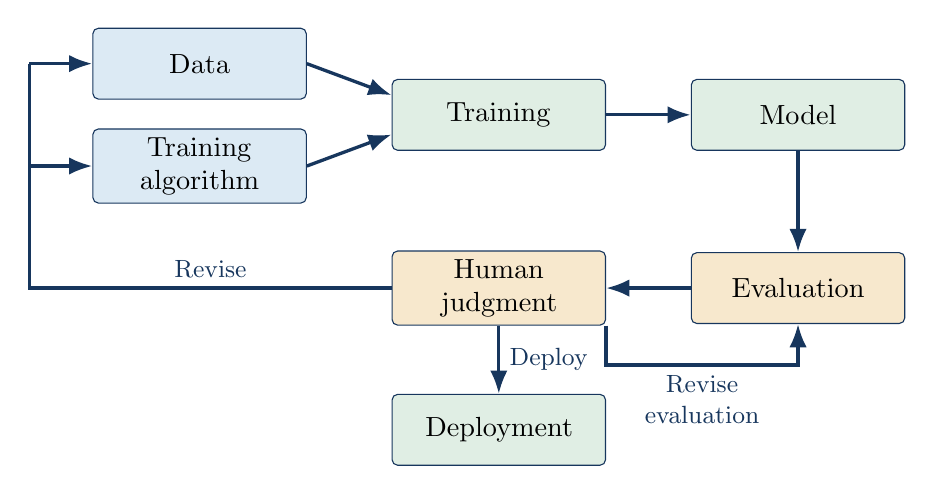
\begin{tikzpicture}[
  >=Latex,
  box/.style={draw=courseblue, rounded corners=2pt, minimum height=9mm,
    text width=25mm, align=center, inner sep=3pt},
  flow/.style={->, very thick, courseblue}
]
\node[box,fill=diagramblue] (data) at (-3.8,0.65) {Data};
\node[box,fill=diagramblue] (alg) at (-3.8,-0.65) {Training algorithm};
\node[box,fill=diagramgreen] (train) at (0,0) {Training};
\node[box,fill=diagramgreen] (model) at (3.8,0) {Model};
\node[box,fill=diagramorange] (eval) at (3.8,-2.2)
  {Evaluation};
\node[box,fill=diagramorange] (judgment) at (0,-2.2)
  {Human judgment};
\node[box,fill=diagramgreen] (deploy) at (0,-4.0) {Deployment};
\draw[flow] (data.east) -- ([yshift=2.5mm]train.west);
\draw[flow] (alg.east) -- ([yshift=-2.5mm]train.west);
\draw[flow] (train.east) -- (model.west);
\draw[flow] (model.south) -- (eval.north);
\draw[flow] (eval.west) -- (judgment.east);
\coordinate (feedback) at ([xshift=-8mm]data.west);
\draw[very thick,courseblue] (judgment.west)
  -- node[above,font=\small] {Revise} (feedback |- judgment.west)
  -- (feedback);
\draw[flow] (feedback) -- (data.west);
\draw[flow] (feedback |- alg.west) -- (alg.west);
\draw[flow] (judgment.south) -- node[right,font=\small] {Deploy} (deploy.north);
\coordinate (evalfeedback) at ([yshift=-5mm]judgment.south east);
\draw[flow] (judgment.south east) -- (evalfeedback)
  -- node[below,font=\small,align=center] {Revise\\evaluation}
  (eval.south |- evalfeedback) -- (eval.south);
\end{tikzpicture}
\caption{Evaluation informs human judgment about whether to revise the system
or deploy it. Human judgment can revise the data, algorithm, and evaluation.}
\label{fig:development-loop}
\end{figure}

Evaluation supplies evidence for a development decision. Performance may
improve on some benchmarks and worsen on others. The team weighs these results
against the intended use and decides whether to revise the system or deploy
it. When evaluation results guide revisions, they become part of the
information used to construct the next system.

Evaluation itself develops through use. People notice failures, discover needs
they had not anticipated, and devise new tests. This feedback continually
brings development into closer agreement with what they want the system to
become. Removing human feedback closes that source of guidance. For a stable,
well-specified task, this may be acceptable. When our aims are still taking
shape, however, a system can improve against its existing criteria while
missing what we have come to care about. The development loop when fully automated
is optimizing the benchmarks; the recent OpenAI-Huggingface incident is a
recent reminder of that this optimization may result in unintended outcomes,
a vivid example of the importance of human oversight and responsibility.

\subsection{Pretraining, post-training, and uneven improvements}

\emph{Pretraining} fits a broad predictive model to large collections of data. For a
language model, it supplies linguistic regularities, factual associations,
styles, patterns of reasoning, and many other statistical regularities present
in the training distribution. It does not by itself specify how a deployed
assistant should interpret instructions, refuse requests, use tools, or prefer
one acceptable response over another.

A pretrained language model continues text by drawing on patterns learned
during pretraining---a ``stochastic parrot'' that can imitate many voices and
genres. A question may elicit an answer, further questions, or an imagined
conversation. For example, base GPT-3 responded to a request for a story by
generating more story-writing instructions, and to a question about code by
supplying multiple-choice options. These are plausible continuations of the
text, but they do not fulfil the request.\endnote{The prompts were selected
to illustrate these behaviours. For a longer
continuation, see GPT-2's fictional report about English-speaking unicorns,
with invented scientists and quotations; that example was selected from ten
generated samples. Sources for both examples are given in the
\hyperref[sec:bibliographical-notes]{bibliographical notes}.}

\emph{Post-training} aims to make the pretrained model useful for its intended tasks.
Post-training consumes data of various forms.
Instruction examples teach
desired input--output behavior; preference or reward signals rank possible
responses; task-specific training can target particular capabilities. These
stages exist because next-token prediction and desired deployed behavior are
different objectives, even though post-training acts on a representation built
by pretraining.

These stages raise several issues.

\begin{itemize}[leftmargin=*]
\item Improving coding performance need not improve creative writing on every
  benchmark. Transfer depends on whether the two tasks use shared internal
  structure and whether the update preserves it. With enough capacity and an
  appropriate procedure, simultaneous improvement may be possible. This creates
  a pressure for larger models. Historically people were vary of large models,
  but with the right data, contrary to some beliefs, there is no theoretical
  reason to stay away from large models. Theory predicts that in the worst-case,
  large models with powerful training are a bad choice. This does not mean that
  on a particular problem they will necessarily do poorly.
\item A large model can still overfit an objective, a dataset, or a repeatedly
  consulted benchmark. More parameters change what can be represented; they do
  not remove the distinction between training evidence and fresh evidence.
\item Training data can contain contradictions. A probabilistic model can
  represent competing continuations and uncertain outcomes. It does not decide
  by itself which contradiction should be resolved in which direction; the
  objective, the data, context, and post-training signals determine the
  learned compromise.
\end{itemize}

This is a curse of developing learned systems: we steer their behavior mostly
through indirect interventions---change data, objectives,
architectures, optimization, or feedback and observe what behavior changes.
Why machine learning is excellent for transforming information
about desired behavior into software when there is no other alternative,
machine learning struggles to produce software that meets strict criteria.

An alternative to the indirect interventions is ``brain surgery'' on the learnt models.
Reverse engineering can reveal useful features or computations, but learned
representations are not designed to be easily ``editable'' (let alone
human-readable). Thus, the success of this direct model-surgery tends
to be limited.

\section{The alignment needed for generalization}

Most inputs an AI system will encounter are absent from its training
data. \emph{Generalization} is therefore essential: it is the mechanism by which
finite experience can support behavior on a much larger set of possible
inputs.

The central principle is:

\begin{center}
\fbox{\parbox{0.86\textwidth}{\centering
Learning works on unseen inputs when the target, data, learner, and information
protocol share exploitable structure.}}
\end{center}

Theory abstracts away details so that we can identify assumptions and derive
their consequences. A proved theorem remains true under its assumptions as
hardware, methods, and research fashions change. Its usefulness for a particular
system depends on what the abstraction leaves out. Some differences change the
conclusion; others have little practical effect. Learning to judge which
differences matter is a central aim of this course. We begin with a simple
learning setting in which we can determine exactly what permits generalization
and what prevents it.

\section{What's in a box? A simple model of learning}
\label{sec:boxes}

There are $N$ boxes numbered $1,\ldots,N$. Each box contains one hidden bit.
The complete collection of bits is given by a fixed but unknown function
\[
f:[N]\longrightarrow\{0,1\},
\qquad [N]:=\{1,\ldots,N\}.
\]
Thus $f(x)$ is the bit in box $x$. The notation
$\{0,1\}^{[N]}$ denotes the set of all such functions. Listing the values
$(f(1),\ldots,f(N))$ identifies the same object with a vector in
$\{0,1\}^N = \underbrace{\{0,1\}\times \dots \times \{0,1\}}_{N \text{ times}}$.

A randomized sampling procedure selects \emph{training} indices
$X_1,\ldots,X_n$ and one \emph{test} index $X$.
The complete tuple
\[
(X_1,\ldots,X_n,X)
\]
produced by the randomized procedure may have \emph{any} joint distribution
on $[N]^{n+1}$.
In particular, the indices may be dependent and may repeat.
The procedure for selecting the indices can be made known to the learner.
The procedure for selecting the indices does not use the hidden labeling
function $f$, so the selected indices cannot themselves communicate
information about the target.

The learner is shown the contents of the boxes with indices $X_1,\dots,X_n$.
No other information is revealed.
Based on this information, the learner must be prepared to
choose a bit for each of the boxes.
After this choice is made, this choice is evaluated on the
test index $X$. The evaluation simply compares the result with $f(X)$.
In case of a match, the learner succeeds, otherwise it suffers a unit loss.
Formally, if $\hat Y\in \{0,1\}$ is the bit that is to be compared to $f(X)$,
the learner's loss is $0$ when $\hat Y = f(x)$ and is $1$, otherwise.
Formally, we can write that the learner's loss is
\begin{align}
\I( \hat Y \ne f(X) )\,. \label{eq:loss}
\end{align}
Here, $\I$ is the so-called \emph{indicator function}. Its argument should be
an event $E$. In particular, for any event $E$, we have
\[
\I\{E\}=\begin{cases}
1,&\text{if $E$ is true}\,;\\
0,&\text{if $E$ is false}\,.
\end{cases}
\]
Strictly speaking, in \cref{eq:loss} we should therefore have used
$\{\hat Y \ne f(X)\}$ as the argument of the indicator function; that is, we
should have written $\I(\{\hat Y \ne f(X)\})$. This is visually
cumbersome, so we abuse notation by dropping the opening and closing braces.
We also do this when we write arguments
of the probability function $\P$. These are standard notational abuses
in probability, and we will continue to use them. One should nevertheless
recognize them as abuses of notation.
The loss in \cref{eq:loss} is called the \emph{$0$--$1$ loss} of predicting $\hat Y$ when the truth is $f(X)$.
This terminology will make more sense as we introduce other losses later.

Since $X$ and $\hat Y$ are random, the loss in \cref{eq:loss} is also random.
To obtain a single numerical measure of the learner's performance, we take the
expectation of this random loss. This gives the learner's expected loss,
$\mathbb E[\I(\hat Y \ne f(X))]$.
A basic property of expectations is that $\mathbb E[\mathbb{I}(E)] = \P(E)$. In words, the expected
value of the indicator of an event is the probability of that event.

In learning terminology, a box index is an \emph{input}, and its hidden bit is
its \emph{label}. Each revealed index--bit pair is a \emph{labeled example}.
The ordered collection of $n$ examples is the \emph{training sample}, also
called the \emph{training data}; repeated inputs are allowed. The \emph{test input}
is the index at which the learner is asked to predict a label.

\paragraph{Combinatorial explosions and asymptopia}
In this example,
each box represents a possible input to some AI system.
If we consider a chatbot that needs to provide yes/no answers to some questions
and we use
a transformer with a maximum context window length $L$ of only $1,000$,
with a (typical) token-vocabulary size of $10^5$, we find that the number
of possible inputs $N$ is
more than $10^{5000}$. This is far more than the number of atoms in the observable
universe.\endnote{Only a tiny fraction of these sequences will take the form of sensible text.
Even questions of the form ``Is the integer with binary representation $b$
divisible by three?'' give $2^{300}>10^{90}$ distinct meaningful inputs when
$b$ ranges over 300-bit strings. With an encoding using at most one token per
binary digit, these questions fit comfortably within the context window.
}
The rapid (exponential) growth of the number of possible inputs by scaling some parameter such as
$L$ is called a \emph{combinatorial explosion}.
Observing every possible input is out of reach.
Even with internet scale data, the number of training data points $n$ is a
vanishing fraction of all possible inputs.
As such, to get a successful AI system,
learning must transfer information from a vanishingly small fraction
of the inputs to the rest of the input space.

\emph{Asymptotic analysis} studies how quantities behave as parameters such as $N$
grow without bound. It can reveal trends that are hard to see in a detailed
finite calculation. For example, exponential and polynomial growth in runtime
have very different consequences as the input size increases. Applying this
guidance requires checking which parameter grows, what is held fixed, and
whether the limiting behavior describes the regime of interest. Constants and
lower-order terms can still matter there. Even an enormous $N$ does not by
itself settle these questions: here, the amount of data and the structure of
the labels will also matter. Explicit finite bounds help us make this judgment.

\subsection{Randomized learners and risk}
We will now formalize what a learner can do. First, consider learners that do
not randomize. Given a labeled sample consisting of $n$ index--bit pairs, such
a learner chooses which bit to assign to each future index.
Formally, we can view such a learner as mapping an element of
$([N]\times \{0,1\})^n$ to $\{0,1\}^{[N]}$ (equivalently, to
$\{0,1\}^N = \underbrace{\{0,1\}\times \dots \times \{0,1\}}_{N\text{ times}}$).
In addition to an $n$-tuple of index--bit pairs, a \emph{randomized learner} takes a
\emph{random seed} $W$ that is uniformly distributed over $[0,1]$.
In \cref{ex:random-seed}, you will show that this choice places no restriction
on the learner's output distribution.
Formally, such a learner can be identified with a measurable deterministic map
\begin{equation}
\cA:\bigl([N]\times\{0,1\}\bigr)^n\times[0,1]
\longrightarrow \{0,1\}^{[N]}.
\label{eq:randomized-algorithm}
\end{equation}

For $(s,w)\in ([N]\times \{0,1\})^n \times [0,1]$, $\cA(s,w)$ is thus a
function from $[N]$ to $\{0,1\}$.
The prediction at the \emph{test index} $X$ is
$\hat Y = \cA(S_f,W)(X)$, where
\begin{equation}
S_f=\bigl((X_i,f(X_i))\bigr)_{i=1}^n
\label{eq:sample}
\end{equation}
is the labeled sample the learner receives before making a decision.\endnote{\textbf{Function application.}
We could write $(\cA(S_f,W))(X)$ instead of $\cA(S_f,W)(X)$ to emphasize that
$\cA(S_f,W)$ is evaluated first and the resulting function is then evaluated
at $X$. We will follow the standard convention of omitting the extra
parentheses. This is analogous to curried function application in programming
languages.}\label{rem:learner-function-application}
\begin{figure}[ht]
\centering
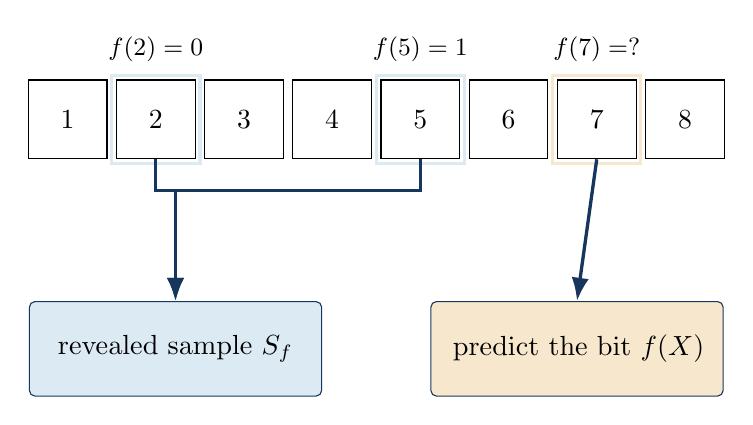
\begin{tikzpicture}[
  >=Latex,
  sample/.style={draw=courseblue,fill=diagramblue,rounded corners=2pt,
    minimum width=12mm,minimum height=9mm,font=\small},
  test/.style={draw=courseblue,fill=diagramorange,rounded corners=2pt,
    minimum width=12mm,minimum height=9mm,font=\small},
  box/.style={draw=courseblue,rounded corners=2pt,align=center,
    minimum height=12mm,text width=35mm,inner sep=3pt},
  flow/.style={->,very thick,courseblue}
]
\foreach \x/\lab in {0/1,1/2,2/3,3/4,4/5,5/6,6/7,7/8}{
  \node[draw,minimum width=10mm,minimum height=10mm] (b\lab) at (\x*1.12,0) {$\lab$};
}
\node[font=\small,above=1mm of b2] {$f(2)=0$};
\node[font=\small,above=1mm of b5] {$f(5)=1$};
\node[font=\small,above=1mm of b7] {$f(7)=?$};
\node[draw=diagramblue,very thick,fit=(b2),inner sep=1.5pt] {};
\node[draw=diagramblue,very thick,fit=(b5),inner sep=1.5pt] {};
\node[draw=diagramorange,very thick,fit=(b7),inner sep=1.5pt] {};
\node[box,fill=diagramblue,below left=18mm and -15mm of b3] (obs)
  {revealed sample $S_f$};
\node[box,fill=diagramorange,below right=18mm and -15mm of b6] (pred)
  {predict the bit $f(X)$};
\draw[flow] (b2.south) -- ++(0,-4mm) -| (obs.north);
\draw[flow] (b5.south) -- ++(0,-4mm) -| (obs.north);
\draw[flow] (b7.south) -- (pred.north);
\end{tikzpicture}
\caption{An example with $N=8$: boxes 2 and 5 were revealed, and box 7 is
the test box. The theorem allows any joint procedure for choosing the revealed
and test indices.}
\label{fig:boxes}
\end{figure}

The expected loss, also known as the \emph{risk}, of the learner that uses
$\cA$, evaluated on a fixed hidden function $f$, is
\begin{equation}
R(\cA,f)=
\mathbb E\!\left[\I\{\cA(S_f,W)(X)\ne f(X)\}\right].
\label{eq:risk}
\end{equation}
Here, the randomness comes from $(X_1,\dots,X_n,X)$ and $W$. Importantly, $W$
is independent of $(X_1,\dots,X_n,X)$. This expresses that the algorithm's
randomization is private.
We suppress the dependence of the risk on the distribution of the random indices
in the notation $R(\cA,f)$ to minimize clutter.

\subsection{Towards robust learners}
Our goal is to make the learner robust. Given $\cA$, we evaluate its performance
under the worst-case choice of $f$. Thus,
$\max_{f\in \{0,1\}^{[N]}} R(\cA,f)$, the \emph{worst-case risk}, is the final performance metric assigned
to a learner that uses $\cA$.
Worst-case analysis is common in computer science: we want protection against
the worst possible case. This is a form of risk aversion or conservatism.
View this as a starting point.
This robust criterion is sometimes viewed as a game: the learner chooses a
procedure, and nature may choose any fixed arrangement of bits. The question is
which method has the smallest worst-case risk.

The critical point is that in \cref{eq:risk}, the test index $X$ either matches
one of the indices $X_1,\dots,X_n$ or matches none of them.
If $X$ matches one of $X_1,\dots,X_n$, the learner should simply use the label
associated with the matching index.
That is, if the learner's data are $((X_1,Y_1), \dots, (X_n,Y_n))$ and $X = X_J$
for some $J\in [n]$, then the learner should set $\hat Y = Y_J$.
This is because \emph{we are promised} that for the (unknown to us) secret function
$f$, $Y_J = f(X_J)$. Thus, choosing $Y_J$, we have $\hat Y = Y_J = f(X_J) = f(X)$.
We are therefore guaranteed to be correct, which gives zero loss, the minimum
possible loss---we are winning!
The challenge is deciding what to do when $X$ matches none of
$X_1,\dots,X_n$.
One may then try to ``figure out some pattern''
in the data and follow that pattern. If we had more structure in the problem,
this could work (more about this soon).
Alternatively, one could simply always return zero or always return one.
One optimal solution is to flip an unbiased coin and return $0$ for heads and
$1$ for tails.
To express this algorithm using the random seed $W$, set
$\hat Y = \mathbb{I}(W\le 1/2)$ when
$X$ is not found in $\{X_1,\dots,X_n\}$.
We will call this algorithm $\cAmem$.

\section{Exact solution of the unstructured boxes problem}
\label{sec:theorem-statement}

Define the event
\begin{equation}
U=\{X\notin\{X_1,\ldots,X_n\}\}\,.
\label{eq:unseen-event}
\end{equation}
This event occurs when the test index does not appear among the indices for
which we have information about the secret function $f$. This is the difficult
case for the learner.
On $U^c$, the learner has been shown the requested bit and can remember it.
On $U$, no revealed label gives direct information about $f(X)$.

The smallest worst-case risk over the allowed learners is the \emph{minimax risk}.

\begin{theorem}[Arbitrary-labeling minimax risk]
\label{thm:arbitrary-labels}
Consider any index-selection procedure allowed in the boxes problem, and let
the learner's random seed $W$ be independent of the selected indices.
Minimizing over the randomized learners defined in
\cref{eq:randomized-algorithm},
\begin{equation}
\min_{\cA}\ \max_{f\in\{0,1\}^{[N]}} R(\cA,f)
=\frac12\P(U).
\label{eq:minimax-risk}
\end{equation}
Furthermore, $\cAmem$ is optimal, that is, it achieves
the above minimax risk.
\end{theorem}

The theorem should be intuitive:
Conditional on seeing the contents of the box
opened at test time, the best loss is zero.
Conditional on not seeing it, the exact minimax loss is $1/2$.
The minimax risk is therefore entirely controlled by the
probability of an unseen box.\endnote{\textbf{Deterministic minimax learners.}
A fair coin attains the minimax value for every allowed sampling law.
Some fixed sampling laws also admit deterministic minimax learners;
\cref{ex:deterministic-minimax} gives an example.}\label{rem:deterministic-minimax}

\Cref{eq:minimax-risk} says two things. There is a learner whose risk is at
most $\tfrac12\P(U)$, however $f$ is chosen. Conversely, for every learner,
there is a labeling function $f$ for which its risk is at least
$\tfrac12\P(U)$.

\subsection{The same boxes, with one shared label}
\label{sec:constant-boxes}

It is instructive to consider the following promise: all boxes contain the same
bit.
Opening any one box now determines every label. For $n\ge1$, the learner
that returns the first observed label at every input has zero risk, even if
the test box has never been opened and $N$ is enormous.

The observation supplies the value of the shared bit. The promise supplies
the relation that makes this value informative about every other box. Thus
the learner receives information both from the observed label and from the
specified target class. The arbitrary-labeling theorem permits $2^N$ targets;
the common-label promise permits only two. \cref{sec:structure} develops
a richer promise for the same boxes question.

Under a structural promise, which boxes are observed can matter more than
how many are observed; see \cref{ex:data-coverage}. This exercise thus illustrates
the utility of having the right type of data.

\subsection{Private randomization and risk}

The order of choices is part of the theorem. Nature may know the algorithm,
but it chooses a fixed $f$ before the learner's seed $W$ is drawn. If nature
could instead choose the unseen test bit after seeing the prediction, it
could force an error by choosing the opposite bit.

\begin{remark}[Risk and repeated experiments]
\label{rem:risk-repetitions}
Random prediction does not promise half an error on one trial. If $E_t$ is the
error indicator in repetition $t$ and the repetitions are independent under
the same $f$ and the same procedure, then the following convergence holds
(\emph{why?}; see \cref{ex:repeated-experiments}).
\[
\frac1T\sum_{t=1}^T E_t \longrightarrow R(\cA,f)
\qquad\text{almost surely}.
\]
This is the operational meaning of risk as a long-run error rate.
\end{remark}

\section{Proof of Theorem~\ref{thm:arbitrary-labels}}
\label{sec:proof}

We give the main argument here in a compact form. A line-by-line version is
given in \cref{app:detailed-proof}. That appendix also explains why
learning to supply the omitted steps is important. The elementary probability
facts used in both versions are reviewed separately in
\cref{app:probability}. Supply the missing justifications in
\cref{ex:complete-boxes-proof}; the expanded proof in
\cref{app:detailed-proof} provides intermediate steps.

We prove the equality by bounding its left-hand side (LHS) both above and
below by its right-hand side (RHS).
For the upper bound, we analyze the particular learner $\cAmem$. For the lower
bound, we fix an arbitrary learner and show that some fixed hidden function
must be hard for it.

\paragraph{Upper bound.}
We first show that the LHS is upper bounded by the RHS. First notice that
\[
\min_{\cA}\max_f R(\cA,f)
\le \max_f R(\cAmem,f)\,.
\]
Now fix some $f\in\{0,1\}^{[N]}$. We will show that
$R(\cAmem,f)=\P(U)/2$. Once this has been shown for every fixed $f$, the upper
bound follows.

For this fixed target $f$, let
$E_f=\{\cAmem(S_f,W)(X)\ne f(X)\}$
be the event that $\cAmem$ makes an error. From the definition of $R$ in
\cref{eq:risk},
\begin{equation}
R(\cAmem,f)
=\P(E_f)
=\P(E_f,U^c)+\P(E_f,U)\,.
\label{eq:upper-split}
\end{equation}

On $U^c$, the test index agrees with at least one training index: $X=X_J$ for
some $J\in[n]$. The learner returns the revealed label
$f(X_J)=f(X)$, so $E_f$ cannot occur. Thus,
\[
E_f\cap U^c=\emptyset,
\qquad
\P(E_f,U^c)=0\,.
\]

On $U$, the learner predicts with the fair bit
$B=\I\{W\le 1/2\}$.
Write $Z=(X,X_1,\ldots,X_n)$.
Conditional on any fixed index tuple $z=(x,x_1,\ldots,x_n)$ that has positive
probability and for which $U$ occurs, $f(x)$ is a fixed bit, whereas $B$ is an
independent fair bit.
Therefore
\[
\P(B\ne f(x)\mid Z=z)=\frac12.
\]
Averaging over the index tuples for which $U$ occurs gives
$\P(E_f,U)=\P(U)/2$. Substituting the two terms into
\cref{eq:upper-split} gives
\begin{equation}
R(\cAmem,f)=\frac12\P(U),
\label{eq:upper-bound}
\end{equation}
for every fixed $f$, which proves the upper bound.

\paragraph{Lower bound.}
We now turn to showing that the LHS is lower bounded by the RHS. Fix an
arbitrary randomized learner $\cA$.
It suffices to prove that $\max_{f\in \{0,1\}^{[N]}} R(\cA,f) \ge \frac12 \P(U)$.
Write $Z=(X,X_1,\ldots,X_n)$. Introduce an auxiliary random function
\[
F:[N]\longrightarrow\{0,1\}
\]
by choosing the bits $F(1),\ldots,F(N)$ independently, with
\[
\P(F(j)=0)=\P(F(j)=1)=\frac12,
\qquad j\in[N].
\]
Choose $F$ independently of the index tuple $(X,X_1,\ldots,X_n)$ and the
learner's seed $W$. Set
\[
\widehat Y=\cA(S_F,W)(X).
\]
We then have
\begin{align}
\max_f R(\cA,f)
&\ge \mathbb E\bigl[R(\cA,F)\bigr]
=\P\bigl(\widehat Y\ne F(X)\bigr)
\ge \P\bigl(\widehat Y\ne F(X),U\bigr)
\label{eq:lower-forward-start}
\end{align}
To continue from the last term in \cref{eq:lower-forward-start}, let
\[
\cZ=
\left\{z=(x,x_1,\ldots,x_n)\in[N]^{n+1}:
x\notin\{x_1,\ldots,x_n\}\right\}.
\]
Fix $z=(x,x_1,\ldots,x_n)\in\cZ$, a possible sample $s$, and
$a,b\in\{0,1\}$. On $\{Z=z,S_F=s\}$, the prediction is
$\cA(s,W)(x)$. The event $\{Z=z,S_F=s\}$ is determined by $Z$ and
coordinates $F(j)$ with $j\ne x$. Hence the independent fair bit $F(x)$
is independent of this event and of $\cA(s,W)(x)$. Consequently,
\begin{align}
&\P\bigl(\widehat Y=a,F(x)=b,Z=z,S_F=s\bigr)\notag\\
&\qquad=\frac12\P\bigl(\widehat Y=a,Z=z,S_F=s\bigr).
\label{eq:unconditional-hidden-bit}
\end{align}
This identity also holds when $\P(Z=z,S_F=s)=0$. Summing the two disjoint
mismatch cases and then all possible $(z,s)$ gives
\begin{align*}
\P\bigl(\widehat Y\ne F(X),U\bigr)
&=\frac12\sum_{z\in\cZ}\sum_s
\left[
\P(\widehat Y=1,Z=z,S_F=s)
+\P(\widehat Y=0,Z=z,S_F=s)
\right]\\
&=\frac12\sum_{z\in\cZ}\sum_s\P(Z=z,S_F=s)
=\frac12\sum_{z\in\cZ}\P(Z=z)
=\frac12\P(U).
\end{align*}
Combining this with \cref{eq:lower-forward-start},
we get $\max_f R(\cA,f)\ge \P(U)/2$. Since $\cA$ was arbitrary, this proves
the lower bound.
\qed

\begin{remark}[Random targets in the lower-bound proof]
\label{rem:random-target-proof}
The random function $F$ is only a device for proving that some fixed target
$f$ must be hard. \cref{sec:optional-reading} returns to this device
and uses it to compare Bayesian and minimax decision making.
\end{remark}

\section{Calculating the unseen probability in an i.i.d. example}
\label{sec:iid}

The theorem allows \emph{dependent} data
(meaning, the joint distribution of $(X_1,\dots,X_n,X)$ is arbitrary; the random variables in it can ``depend'' on each other).
We now add a special assumption to
obtain a closed form: $X_1,\ldots,X_n,X$ are independent
draws from the same distribution $P$ on $[N]$. Write $P(x)$ for the
probability assigned to index $x$.
Besides this giving us a closed form, the  assumption models a scenario
which is often not a bad approximation of reality:
The data collection and the testing follows a random process,
and the data points are chosen independently of each other.
For example, if physical experiments are used to obtain a data point,
these experiments are somehow isolated from each other in time and space,
so the randomness that governs the outcome of obtaining the first datapoint
does not influence that of the second.

When running experiments in a lab, this is where the equipment would not be
``reset'' to its pristine state, all conditions controlled.
When collecting survey data, this is where the telephone numbers of people
chosen to be surveyed should be chosen by throwing that $N$-sides
dice independently of each other (most likely, using a computer, pretending
computers produce real randomness). Stopping people at a shopping mall
and talking to them will not produce an independent sample (couples often
shop together, people go to a shop at a certain time may have similar jobs),
let alone one that is uniform. The characters of a text are definitely not independent
of each other by any means. The \emph{i.i.d.} (\emph{independent, identically distributed})
assumption is common as it allows some crude quantification of
how information scales with data, as we will illustrate now. We will return to going beyond this assumption later.
An important detail of this assumption that the test index is drawn from the same distribution
as the training indices. The meaning of this is that deployment data is obtained the same way as test data.
This is again often not true; when this does not hold, we talk about \emph{distribution shift} (more specifically, \emph{covariate shift}, since
the inputs, with an old word from statistics are also called \emph{covariates}).
TODO: Add a simple exercise about covariate shift; probability ratios govern how much the error shifts.

Conditioning on $X=x$ gives
(see \cref{ex:unseen-probability})
\begin{equation}
\P(U)=\sum_{x=1}^N P(x)(1-P(x))^n.
\label{eq:unseen-iid}
\end{equation}
If $P$ is uniform, then
\begin{equation}
\P(U)=\left(1-\frac1N\right)^n,
\qquad
\min_{\cA}\max_f R(\cA,f)
=\frac12\left(1-\frac1N\right)^n.
\label{eq:uniform-risk}
\end{equation}
For fixed $N$, the risk tends to zero as $n$ grows. But when $n/N$ is small,
it remains close to $1/2$: eventual coverage does not help in this regime.

For example, a sufficient condition for worst-case risk at most $0.1$ is
\begin{equation}
n\ge N\log 5,
\label{eq:sample-upper}
\end{equation}
because $(1-1/N)^n\le e^{-n/N}$. Conversely, Bernoulli's inequality gives
$(1-1/N)^n\ge 1-n/N$, so risk at most $0.1$ requires $n\ge0.8N$.
\Cref{ex:sample-size-bounds} asks you to prove both inequalities and derive
these sample-size bounds.
Thus an unstructured problem with independent uniform training and test
indices requires a number of observations proportional to the number of
boxes. When $N$ is enormous relative to $n$, almost every test input remains
unseen, and achieving, say, $n\ge 0.8 N$ is hopeless.

\section{What's in a box? Part II: a threshold promise}
\label{sec:structure}

We keep the boxes, the observations, and the prediction question. As in the
common-label example, we change the promise about their contents.
In that example, we assumed that the labeling functions $f:[N]\to \{0,1\}$ that
we may ever see are constant. Here, we assume that these functions are nondecreasing
as a function of the box indices: Going from smaller to larger indices, once a label is 1,
all subsequent labels are 1. Equivalently,
$f = f_k$ for some
unknown \emph{threshold} $k\in[N+1]$, where
\begin{equation}
f_k(j)=\I\{j\ge k\},
\qquad j\in[N].
\label{eq:threshold}
\end{equation}
(The case $k=N+1$ is the all-zero function.)
One observed positive label now
constrains every box to its right, and one observed negative label constrains
every box to its left. Information transfers between different inputs.

Just like in the previous section,
for the quantitative bound below, assume that the training indices and the
test index are independent draws from the same probability distribution $P$
on $[N]$. Again, we will write $P(x)$ for the probability assigned to index $x$.
This assumption ensures that a region with substantial test probability also has
a substantial chance of being represented in the training data.
\Cref{ex:threshold-sampling} explores what can be proved under more general
sampling assumptions.

\newcommand{\kest}{K}
Let $\kest$ be the smallest index with an
observed positive label, and set $\kest=N+1$ if no positive label was
observed. The learner returns $f_{\kest}$.
Assume that the true labeling function (unknown to the learner) is $f_k$.
The chance that the learner is missing the correct label on the test index $X$
given the training indices $(X_1,\dots,X_n)$ is
\begin{equation}
M=\P(f_\kest(X)\ne f_k(X)| X_1,\dots,X_n)\,.
\label{eq:threshold-risk}
\end{equation}
We will call this the \emph{error mass} on a fresh sample from $P$.
It follows from the definition that
\[
M = \sum_{x=1}^N P(x)\I\{f_{\kest}(x)\ne f_k(x)\}.
\]
The error mass is therefore a random variable
through $\kest$, whose randomness comes from that of $X_1,\dots,X_n$.
The next proposition shows that the chance of this random
error exceeding some level $\epsilon$ decreases exponentially fast in $n$
(to be precise, in $n\epsilon$):

\begin{proposition}[Threshold generalization]
\label{prop:threshold}
For every $P$, every threshold $f_k$, and every $\epsilon\in(0,1)$,
\begin{equation}
\P\bigl(M>\epsilon\bigr)
\le (1-\epsilon)^n
\le e^{-n\epsilon}.
\label{eq:threshold-bound}
\end{equation}
Consequently, $n\ge \epsilon^{-1}\log(1/\delta)$
observations suffice to guarantee that the error mass stays below $\epsilon$
with probability exceeding $1-\delta$.
\end{proposition}
Note how the threshold to guarantee a small error mass is independent of $N$.

\begin{proof}
If $k=N+1$, every label is zero, the learner is exact, and the claim is
immediate. Assume therefore in the rest of the proof that $k\le N$.
The learner chooses $K$ to be the smallest index with a positive label if such an index
exists, otherwise it chooses $K=N+1$.
Because of this, we claim that the learner
makes a mistake exactly when tested at an index in the interval $[k,K) := \{k,k+1,\dots,K-1\}$ (in this proof
intervals are restricted to integers in the interval).

First, notice that $K\ge k$ always holds, so this interval is well-defined (it could be empty when $K=k$).
Indeed, if there was no positive label, $K=N+1\ge k$, while if there is a positive label,
$f_k(K)=1$, which is only possible if $K\ge k$ by the definition of $f_k$.

Now, since $K\ge k$ always holds, that is, the learner is overestimating the index $k$,
the learner predicts all $0$ labels correctly and it also predicts all $1$ labels correctly
for indices at least $K$. For any of the indices $x$ in $[k,K)$, $f_k(x)=1\ne 0=f_K(x)$,
establishing the claim.

Hence, $M = \sum_x P(x) \I( f_K(x)\ne f_k(x)) = P( [k,K) ) = q(K-1)$
where for $k-1\le j \le N$, we define $q(j) = P([k,j])$, with
$[k,k-1]=\emptyset$, so $q(k-1)=0$.
Clearly, this function is nondecreasing on $[k-1,N]$.

If $q(N)\le \epsilon$, $\P(M>\epsilon)=0$ and the result holds. Therefore assume
that $q(N)>\epsilon$ and let $j_\epsilon$ be the smallest index $k\le j \le N$ such that $q(j)>\epsilon$.
Since $q$ is nondecreasing, $q(j)\le \epsilon$ for every $j<j_\epsilon$ and
$q(j)> \epsilon$ for every $j\ge j_\epsilon$.
Therefore,
\[
\{M>\epsilon\} = \{q(K-1)>\epsilon\} = \{K>j_\epsilon\}\,.
\]

Now, $K>j_\epsilon$ can only hold if the sample
 $\{X_1,\dots,X_n\}$
 had no point in $[k,j_\epsilon]$ (otherwise, at the point in this interval the label would be one,
 forcing $K$ to be at most $j_\epsilon$).
Thus,
\begin{equation}
\{ K>j_\epsilon \} \subset \{ X_1\not\in [k,j_\epsilon]\} \cap \dots \cap \{ X_n\not\in [k,j_\epsilon]\}\,.
\label{eq:threshold-missed-interval}
\end{equation}
Taking probabilities and using that $X_1,\dots,X_n$ are independent and identically distributed, we get
\[
\P(M>\epsilon) = \P(K>j_\epsilon) \le \P(X_1\not\in [k,j_\epsilon])^n\,.
\]
Now, $\P(X_1\not\in [k,j_\epsilon]) = 1-\P(X_1\in [k,j_\epsilon])$ and since
$\P(X_1\in [k,j_\epsilon])=P([k,j_\epsilon])=q(j_\epsilon)>\epsilon$,
$\P(X_1\not\in [k,j_\epsilon])<1-\epsilon$.
Chaining the inequalities gives the first inequality,
while the second follows by the elementary inequality that $\log(1+x)\le x$ which holds for all $x>-1$.\endnote{\textbf{The exact threshold tail.}
The inclusion in \cref{eq:threshold-missed-interval} is actually an equality.
Indeed, if the sample misses $[k,j_\epsilon]$, every observed positive index
must exceed $j_\epsilon$. Thus, when $q(N)>\epsilon$, the exact error-tail
probability is
\[
\P(M>\epsilon)=(1-q(j_\epsilon))^n.
\]
When $q(N)\le\epsilon$, this probability is zero.}\label{rem:threshold-exact-tail}
\end{proof}


\subsection{Comparing expected error in the same boxes problem}

The boxes theorem bounds risk averaged over the sample, test input, and
learner's randomization. The threshold proposition gives a stronger kind of
control: it bounds the probability that the learned predictor's error mass
exceeds a specified level. This also yields an expected-risk bound.

\begin{corollary}[Expected risk of the threshold learner]
\label{cor:threshold-expected}
For every distribution $P$ on $[N]$, every threshold target $f_k$ with
$k\in[N+1]$, and every
sample size $n\ge0$, let the training and test indices be independent draws
from $P$. The risk of the learner returning $f_K$ satisfies
\begin{equation}
\mathbb E[M]\le\frac{1}{n+1}.
\label{eq:threshold-expected}
\end{equation}
\end{corollary}

\Cref{ex:threshold-expectation} asks you to derive this corollary from
\cref{prop:threshold} by integrating the tail probability in
\cref{eq:threshold-bound}.

For a direct comparison, use independent uniform training and test indices
in both problems. Allowing arbitrary labels gives exact minimax risk
$\tfrac12(1-1/N)^n$, so expected error at most $0.1$ requires $n\ge0.8N$.
With the threshold promise, $n=9$ already suffices for expected error at most
$0.1$, for every $N$. This upper bound even holds for every input distribution
$P$. With the common-label promise, one observation suffices for zero error.

\subsection{Hypothesis classes and beyond}
\label{sec:hypothesis-classes}

All three boxes problems ask what can be predicted about closed boxes from
open ones. Their different answers come from different promises about the
target: it may be any function, a constant function, or a threshold. We can
express such a promise by specifying a set of possible targets.

\begin{definition}[Realizability and consistency]
\label{def:realizability-consistency}
Let $\cF\subseteq\{0,1\}^{[N]}$ be a nonempty \emph{target class}.
The assumption that the true labeling function $f$ belongs to $\cF$ is
called \emph{realizability}. A predictor $g$ is \emph{consistent} with a
labeled sample $((x_i,y_i))_{i=1}^n$ if $g(x_i)=y_i$ for every $i$.
\end{definition}

Such a set of predictors is commonly called a \emph{hypothesis class}.
The assumption that the target belongs to $\cF$, called \emph{realizability},
does not imply that the learner returns a member of $\cF$. A learner that
always returns a member of $\cF$ is called \emph{proper}; otherwise it is
called \emph{improper}. This is peculiar terminology: there is nothing
improper about improper learning.

The next theorem assumes realizability and applies to learners that return
a consistent member of $\cF$. Such a member exists because the target $f$
belongs to $\cF$ and agrees with every training label.

For a predictor $g$ and target $f$,
a distribution $P$ over the inputs,
write
\[
L_P(g,f)=\P( g(X)\ne f(X))
\]
where the test point $X$ has distribution $P$ (with symbols, $X\sim P$).
For a learned predictor $\widehat f$,
this is the same as its error mass:
$M=L_P(\widehat f,f)$, extending the notation from the threshold problem.

\begin{theorem}[Generalization by consistency in a finite class]
\label{thm:finite-class-consistency}
Let $\cF\subseteq\{0,1\}^{[N]}$ be nonempty, $f\in\cF$, and let
$X_1,\ldots,X_n$ be independent draws from a distribution $P$ on $[N]$.
Any learner returning a member $\widehat f\in\cF$ consistent with
$((X_i,f(X_i)))_{i=1}^n$ satisfies, for every $\epsilon\in(0,1)$,
\begin{equation}
\P\bigl(L_P(\widehat f,f)>\epsilon\bigr)
\le |\cF|e^{-n\epsilon}.
\label{eq:finite-class-consistency}
\end{equation}
In particular, for $\delta\in(0,1)$,
$n\ge\epsilon^{-1}(\log|\cF|+\log(1/\delta))$ suffices for error mass
at most $\epsilon$ with probability at least $1-\delta$.
\end{theorem}

\Cref{ex:finite-class-consistency} asks you to prove this theorem. It applies
to any choice among consistent members, including a randomized choice.
The restriction to $\cF$ matters: matching observed labels alone gave no
useful prediction on unseen boxes in the unstructured problem. The theorem
also leaves a computational question: how do we find a consistent member
efficiently?

For thresholds, $|\cF|=N+1$, so the cardinality bound introduces a
$\log(N+1)$ term absent from \cref{prop:threshold}. This is a limitation of
counting hypotheses. General theory based on \emph{VC dimension}
recovers the optimal sample-complexity rate for thresholds
without dependence on $N$. Our direct proof gives a simple argument and
explicit constants.

\begin{remark}[Consistency and optimal sample complexity]
\label{rem:erm-optimal-rates}
An \emph{empirical risk minimizer} (ERM) minimizes (average) loss on the
training sample over the hypothesis class. Under realizability and $0$--$1$
loss, this means choosing a consistent member. An arbitrary such choice
need not achieve the optimal sample-complexity rate: some ERM learners
require an extra logarithmic factor. Thus consistency alone does not settle
how to learn with the fewest observations. See
the \hyperref[sec:bibliographical-notes]{bibliographical notes} for
optimal rates and limitations of ERM.
\end{remark}

\paragraph{When the promise fails.}
Realizability requires justification, and for many applications we cannot
justify it. \emph{Label noise} and \emph{misspecification} are different issues: noise
concerns the observed labels, while misspecification means that the assumed
model does not contain the data-generating mechanism. Allowing label noise
does not ensure that the underlying target belongs to a chosen class.

The \emph{agnostic} approach compares the learner's performance with that
of the best predictor in a chosen class, without assuming the class contains
a perfect predictor. This comparison is useful, but a small gap to the best
predictor in the class need not mean good absolute performance. Every member
of the class may perform poorly.

\paragraph{Algorithm design beyond a class.}
Choosing a class is one design choice. It generally does not determine which
predictor to prefer, how to find it, what data to acquire, or which performance
criterion to use. Architecture, optimization, regularization, and data
collection can all affect the result. Later in the course we will study
\emph{algorithmic bias}: the preferences built into a learning procedure,
including its choices among predictors that fit the same observations.

\begin{remark}[Bayesian modeling and design choices]
\label{rem:bayesian-design-choices}
A \emph{prior} supplies weights on possible targets and can express preferences
within a class. Choosing the prior, the loss, and the observation model
remains part of designing the system. \Cref{sec:optional-reading} develops
the Bayesian decision criterion.
\end{remark}

It helps to distinguish two questions. What can a method guarantee across a
specified family of problems? What method should we use for this application,
with this information, objective, and computational budget? General theory
informs the second question; applying it requires judging whether its
assumptions and criterion fit. Even the goal of building a broadly capable AI
system requires choices about what capabilities to seek and how to evaluate
them. Hypothesis classes help us study generalization, but choosing a class
does not settle the broader problem of designing a learning system.

\section{Optional reading: priors, best responses, and robustness}
\label{sec:optional-reading}
\label{app:decision-theory}

The lower-bound proof introduced a random function $F$ to average risks over
possible targets. A distribution over targets can also be used to define a
decision criterion. This leads to two different questions: what minimizes
average risk under a specified prior, and what minimizes worst-case risk?

\subsection{Priors and Bayes rules}
Let $\cF=\{0,1\}^{[N]}$ and let $\pi$ be a probability distribution on
$\cF$. Draw $F$ from $\pi$ independently of the indices and the learner's
seed. A \emph{Bayes rule} minimizes
\begin{equation}
\mathbb E[R(\cA,F)].
\label{eq:bayes-risk}
\end{equation}
This expectation averages over $F$; $R(\cA,f)$ already averages over the
indices and the learner's seed. For a sample $s$ of positive probability,
the \emph{posterior probability} of label 1 at index $x$ is
\[
p(s,x)=\P(F(x)=1\mid S_F=s).
\]
A Bayes rule chooses a prediction to minimize its conditional expected loss.
\Cref{ex:one-bit-decisions} asks you to derive that choice and compare it
with the worst-case choice for an unknown bit.

\begin{remark}[Information supplied by a prior]
\label{rem:prior-information}
The prior supplies weights on possible targets. These weights may encode
knowledge, judgment, or a modeling assumption; they are not selected by the
Bayes optimization itself. Priors can also supply relations between labels:
\cref{ex:prior-structure} compares independent labels with a shared label.
\end{remark}

\subsection{The finite minimax theorem}
Let $\cD$ be the finite set of deterministic learners, and write
$\Delta(\cD)$ and $\Delta(\cF)$ for distributions on learners and targets.
A distribution $\mu\in\Delta(\cD)$ describes a randomized learner.
For independently drawn $A\sim\mu$ and $F\sim\pi$, define
\begin{equation}
L(\mu,\pi)=\mathbb E[R(A,F)].
\label{eq:game-payoff}
\end{equation}
Here $A$ is a random element of $\cD$. Let $\delta_f$ put probability one
on target $f$. The finite minimax theorem gives
\begin{equation}
\min_{\mu\in\Delta(\cD)}\max_{f\in\cF}L(\mu,\delta_f)
=\max_{\pi\in\Delta(\cF)}\min_{\mu\in\Delta(\cD)}L(\mu,\pi).
\label{eq:finite-minimax}
\end{equation}
For each $\pi$, the inner minimum on the right is its \emph{Bayes risk}. A prior
attaining the outer maximum is called \emph{least favorable}. Thus the
optimal worst-case risk equals the largest Bayes risk over priors.
\begin{remark}[Bayes optimality and minimax optimality]
\label{rem:bayes-minimax}
The uniform prior used in the boxes proof is least favorable. The equality
of values does not imply that every Bayes rule for that prior is minimax;
\cref{ex:bayes-not-minimax} asks you to establish both claims.
\end{remark}

\subsection{Performance across sampling laws}
\label{sec:sampling-law-comparison}
Let $\cQ$ be the set of joint distributions of $(X_1,\ldots,X_n,X)$.
Each $Q\in\cQ$ is the same for every hidden target. Write $R_Q(\cA,f)$
when the sampling law must be explicit, and define
\begin{equation}
V(Q)=\min_{\cA}\max_{f\in\cF}R_Q(\cA,f)=\frac12 Q(U).
\label{eq:q-specific-value}
\end{equation}
One can seek a learner minimizing the worst risk over both $Q$ and $f$, or
require a learner to attain $V(Q)$ separately for every $Q$. These are
different requirements. \Cref{ex:minimax-regret-q,ex:regret-comparison}
compare the corresponding benchmarks.

\subsection{Choosing a criterion}
A Bayesian model requires a prior; a minimax model requires a class of
possible environments. Both require a loss, an observation protocol, and a
class of allowed decisions. A broad environment class can make a worst-case
guarantee conservative, while a prior can omit important possibilities.
The choice should reflect the question and the information available.

Prefer minimax risk when an absolute performance guarantee is the governing
objective; environment-dependent costs and common fallbacks can then affect
the choice. Prefer \emph{minimax regret} when the objective is to limit avoidable
shortfall relative to available opportunities; the comparator set must then
be specified carefully. If both considerations matter, examine both: small
regret can coexist with large risk, and minimizing worst-case risk can
tolerate avoidable losses in easier environments.
\Cref{ex:risk-versus-regret} explores this choice through common fallbacks
and changes to the available decisions.

\begin{remark}[Which invariance properties should a criterion satisfy?]
\label{rem:criterion-invariance}
Should mixing every decision with the same fallback preserve their ranking?
Should adding a decision that is not chosen preserve the choice among the
original decisions? The calculations in \cref{ex:risk-versus-regret} show
that minimax risk and minimax regret respond differently. Which properties
to insist on depends on the application: whether absolute losses or avoidable
shortfalls matter, and what information the comparator should use.
\end{remark}

\section{Take-home messages}
\label{sec:take-home}

\begin{enumerate}[leftmargin=*,itemsep=0.25em,topsep=0.4em]
\item Machine learning moves part of the behavioral specification problem into
data and feedback. Architecture, objectives, optimization, evaluation, and the
surrounding program remain designed components.
\item Pretraining, post-training, and repeated evaluation supply different
information. A capability should be attributed to the components that made it
possible.
\item In the boxes problem, the training and test indices may have any joint
distribution that is the same for every hidden function, with the learner's
seed independent of the indices. The exact minimax risk is one half of the
probability that the test index was not revealed.
\item Private randomization protects an unseen prediction against a fixed
worst-case label. It creates no information about that label.
\item Generalization requires alignment: the learner and its observations must
exploit relations that the target actually satisfies.
\item Finite input spaces can be astronomically large. Interpret asymptotic
guarantees in the relevant regime, and inspect their explicit dependence on
sample size, domain size, and the promised structure.
\end{enumerate}

\printendnotes

\section*{Bibliographical notes}
\phantomsection
\label{sec:bibliographical-notes}

\paragraph{Pretraining examples.}
The base GPT-3 continuations discussed in the text appear in
\href{https://arxiv.org/html/2203.02155v1\#S4.F8}{Figure 8 of Ouyang et al. (2022)}.
The prompts were selected to illustrate those behaviours.
GPT-2's fictional report about English-speaking unicorns appears in
\href{https://cdn.openai.com/better-language-models/language_models_are_unsupervised_multitask_learners.pdf\#page=20}{Table 13 of Radford et al. (2019)};
that example was selected from ten generated samples.

\paragraph{Counting possible inputs.}
For the comparison with the number of atoms in the observable universe, see
Peter Norvig,
\href{https://www.norvig.com/atoms.html}{\emph{On the (Small) Number of Atoms
in the Universe}} (2016).

\paragraph{Probability.}
The conventions for random variables, vectors, and elements follow
\href{https://tor-lattimore.com/downloads/book/book.pdf}{Lattimore and
Szepesv\'ari, \emph{Bandit Algorithms}}, Chapter~2. That chapter develops
probability spaces, measurability, conditioning, and independence in greater
generality. \Cref{app:probability} collects the tools needed here.

\paragraph{Randomized algorithms.}
Randomized algorithms are a major subject in theoretical computer science.
Their mathematical analysis typically assumes access to independent random
bits. Software commonly uses pseudorandom generators, which deterministically
expand a seed into a longer sequence; whether this adequately replaces ideal
randomness depends on the application and assumptions. See Motwani and
Raghavan, \emph{Randomized Algorithms}, and Vadhan,
\href{https://people.seas.harvard.edu/~salil/pseudorandomness/}{\emph{Pseudorandomness}}.

\paragraph{Hypothesis classes, realizability, and ERM.}
Shalev-Shwartz and Ben-David's
\href{https://www.cs.huji.ac.il/~shais/UnderstandingMachineLearning/understanding-machine-learning-theory-algorithms.pdf}{\emph{Understanding
Machine Learning: From Theory to Algorithms}} (2014), Chapters~2--4,
develops realizability, consistency, ERM, and finite-class guarantees.
Remark~3.2 discusses proper versus improper learning; the terminology
``hypothesis class'' does not by itself restrict the learner's output.
Section~5.2 separates approximation error from estimation error, clarifying
why approaching the best predictor in a class need not give small absolute
risk. Chapter~6 introduces VC dimension and the classical learnability
characterization. The optimal-rate results below postdate that textbook.

\paragraph{VC dimension and optimal sample complexity.}
For a class of VC dimension $d$, Hanneke's
\href{https://jmlr.org/papers/v17/15-389.html}{\emph{The Optimal Sample
Complexity of PAC Learning}} (2016) gives a realizable PAC learner using
$O((d+\log(1/\delta))/\epsilon)$ observations. This removes the extra
$\log(1/\epsilon)$ factor in the classical guarantee for arbitrary ERM
learners. The algorithm combines consistent predictors by majority vote and
may return a predictor outside the original class.

\paragraph{When improper learning helps.}
The distinction can affect the best achievable sample complexity, even
without computational restrictions. Bousquet, Hanneke, Moran, and
Zhivotovskiy's
\href{https://proceedings.mlr.press/v125/bousquet20a.html}{\emph{Proper
Learning, Helly Number, and an Optimal SVM Bound}} (2020),
\href{https://proceedings.mlr.press/v125/bousquet20a/bousquet20a.pdf\#page=10}{Theorem~11},
exhibits classes for which \emph{every} proper learner needs an additional
logarithmic factor. This is stronger than showing that some ERM choices
are inefficient in their use of data.

The finite singleton class in its proof gives a boxes example: exactly one
of $N$ boxes is positive. A proper learner must designate one box as
positive. If sampling is uniform over the other $N-1$ boxes, reliable
identification of the missing box requires order $N\log N$ observations.
An improper learner can return the all-zero predictor until a positive label
is observed, then return the identified singleton. For any $P$, this rule's
error exceeds $\epsilon$ only if the positive box has mass greater than
$\epsilon$ and is missed in every draw, an event of probability at most
$e^{-n\epsilon}$. At $\epsilon=1/(2(N-1))$ and fixed small failure
probability, it therefore needs only order $N$ observations. The gain comes
from allowing a prediction that need not assert an unobserved positive label.

\paragraph{Transduction.}
Transduction can save labels when the unlabeled test inputs reveal structure
that constrains their labels. Examples include
\href{https://www.cs.cmu.edu/~zhuxj/pub/zgl.pdf}{graph-based label propagation},
which encourages similar inputs to share labels, and
\href{https://www.cs.cornell.edu/people/tj/publications/joachims_99c.pdf}{transductive SVMs},
which seek a large margin on labeled and unlabeled examples. In learning
theory, the
\href{https://arxiv.org/abs/2212.09270}{one-inclusion graph algorithm}
is central; its transductive analysis also yields inductive expected-risk
guarantees. Label savings are not universal: for distribution-free, realizable
binary classification with i.i.d. training and test samples and at least as
many test as training examples, the optimal labeled-sample complexity has the
same order in transduction and induction. See
\href{https://arxiv.org/abs/1602.03027}{Tolstikhin and Lopez-Paz (2016)}.

\paragraph{Decision criteria.}
For axiomatic treatments, see Stoye's
\href{https://stoye.economics.cornell.edu/docs/AxiomsRegret.pdf}{\emph{Axioms
for Minimax Regret Choice Correspondences}} (2011), and Section~3.2 and
Table~1 of his survey
\href{https://stoye.economics.cornell.edu/docs/ARE.pdf}{\emph{New Perspectives
on Statistical Decisions under Ambiguity}}. These characterizations make
explicit the tradeoffs between consistency requirements; they do not single
out one criterion as universally preferable.


\clearpage

\section*{Glossary}

This glossary collects learning and decision-theory terminology used in the
notes. Basic probability terminology is defined in \cref{app:probability}
and is omitted here.

\begin{description}[style=nextline,leftmargin=1.5em,labelindent=0pt]
\item[Input; label; labeled example]
An input $x$ is an object on which a prediction is requested; its label $y$
is the associated answer. A labeled example is an observed pair $(x,y)$.
In the boxes problem, $x$ is a box index and $y=f(x)$ is its hidden bit.
\item[Training sample]
The observations supplied to the learner. Here
$S_f=((X_i,f(X_i)))_{i=1}^n$ is a tuple of labeled examples; indices may
repeat, and independence is an additional assumption.
\item[Test input]
An input $X$ at which a prediction is evaluated against its label $f(X)$.
Its label is withheld for evaluation, but the same input and label may
already have appeared in the training sample.
\item[Sampling law]
The joint distribution $Q$ of $(X_1,\ldots,X_n,X)$. In the original boxes
problem it may have dependence and repeated indices, but it does not depend
on the hidden target $f$. Independent draws from a common distribution $P$
are a special case; see \cref{sec:boxes,sec:iid}.
\item[Target]
The fixed, unknown function $f$ that supplies the true labels. The noiseless
boxes problem has $f:[N]\to\{0,1\}$.
\item[Predictor]
A function $g$ that assigns a predicted label to an input. A learned
predictor $\widehat f$ depends on the training sample and possibly on
the learner's random seed.
\item[Learner]
A procedure $\cA$ that constructs a predictor from a training sample and
private seed: $\widehat f=\cA(S_f,W)$. The subsequent prediction at $X$
is $\widehat f(X)$; see \cref{eq:randomized-algorithm}.
\item[Generalization]
Using training information to achieve low prediction error on test examples
under a specified evaluation protocol. Test inputs need not be distinct
from training inputs; the guarantees concern performance at test time.
\item[Structural promise]
An assumption restricting the possible targets, such as requiring all labels
to agree or requiring them to form a threshold. Such restrictions can relate
labels at different inputs.
\item[Hypothesis class]
A specified set $\cF$ of candidate prediction functions. The class may be
used to restrict the learner's search or to define a comparison benchmark;
naming it alone does not restrict every learner's output to it.
\item[Target class]
The set of functions allowed as possible targets. The same set $\cF$ may
serve as both a target class and a hypothesis class, but these are different
roles.
\item[Realizability]
In the noiseless setting here, the assumption $f\in\cF$: the specified
class contains the true labeling function. This assumption concerns the
target, not the learner's choice of output.
\item[Consistency]
A predictor $g$ is consistent with a sample $((x_i,y_i))_{i=1}^n$ if
$g(x_i)=y_i$ for every $i$. This is a property of its predictions on the
observed sample.
\item[Empirical risk]
Average loss on the observed training sample. Under $0$--$1$ loss, for
$s=((x_i,y_i))_{i=1}^n$ with $n\ge1$, it is
$\widehat L_s(g)=n^{-1}\sum_{i=1}^n\I\{g(x_i)\ne y_i\}$.
\item[Empirical risk minimization (ERM)]
Choosing $g\in\operatorname*{arg\,min}_{h\in\cF}\widehat L_s(h)$.
Under realizability and noiseless labels, the minimum $0$--$1$ empirical
risk is zero, so every ERM output is consistent. Different choices among
minimizers can have different generalization guarantees.
\item[Proper; improper learning]
A proper learner always returns a member of the class being learned; an
improper learner may return a predictor outside it.
\item[$0$--$1$ loss]
The loss $\I\{\widehat y\ne y\}$ for predicting $\widehat y$ when the
true label is $y$: zero for a correct prediction and one for an error.
\item[Risk]
Expected loss under the specified evaluation protocol. Here
$R(\cA,f)=\mathbb E[\I\{\cA(S_f,W)(X)\ne f(X)\}]$ averages over the
jointly sampled training and test indices and the learner's seed, with $f$
fixed. Writing $R_Q$ makes the sampling law explicit; see \cref{eq:risk}.
\item[Error mass]
For fixed $g$, $f$, and input distribution $P$, the probability assigned
to prediction errors is
$L_P(g,f)=\sum_{x=1}^N P(x)\I\{g(x)\ne f(x)\}$.
For a learned $\widehat f$, the quantity $M=L_P(\widehat f,f)$ is random
through the training data and any private randomization. If the test input
has law $P$ and is independent of both, then
$R(\cA,f)=\mathbb E[M]$, with the expectation over the training data and
the learner's seed.
\item[Unseen input]
A test input whose index is absent from the training sample. In the boxes
problem this is the event $U=\{X\notin\{X_1,\ldots,X_n\}\}$.
\item[Threshold target]
On the ordered inputs $[N]$, the function $f_k(x)=\I\{x\ge k\}$ for
$k\in[N+1]$. The cases $k=1$ and $k=N+1$ give the all-one and all-zero
functions, respectively; see \cref{eq:threshold}.
\item[Worst-case risk]
For a fixed learner and sampling law $Q$, the value
$\max_{f\in\cF}R_Q(\cA,f)$. The target is chosen to maximize expected
loss, without seeing the learner's private random seed.
\item[Minimax risk]
The smallest worst-case risk among allowed learners, here
$\min_{\cA}\max_{f\in\cF}R_Q(\cA,f)$ for fixed $Q$.
The target class and sampling assumptions are part of the criterion;
maximizing over $Q$ as well defines a different optimization problem.
\item[Sample complexity]
The smallest number of training observations for which an allowed learner
can meet a specified guarantee uniformly over the stated targets and
sampling distributions. For example, a high-probability guarantee requires
$\P(M\le\epsilon)\ge1-\delta$; an expected-risk guarantee instead bounds
$\mathbb E[M]$ under the independent-test setup.
\item[Private randomization]
The learner's seed $W$ is independent of the sampled indices, and the target
is chosen without access to it. The learner may use $W$ together with its
observations to randomize its predictions.
\item[Label noise]
Randomness or corruption in observed labels, so that they need not equal
the value of a fixed labeling function at the observed input.
\item[Misspecification]
Failure of the assumed model class to contain the data-generating mechanism.
In the noiseless function setting, this means $f\notin\cF$.
\item[Agnostic learning]
Learning with a guarantee relative to the best predictor in a specified
class, without assuming that any member predicts perfectly. The comparison
controls excess risk over that class's best risk, which may itself be large.
\item[Algorithmic bias]
Preferences built into a learning procedure, including its choices among
predictors that fit the same observations.
\item[Inductive learning]
Constructing a predictor from training data before receiving the particular
inputs on which it will be evaluated.
\item[Transductive learning]
Predicting labels for particular unlabeled test inputs that are supplied
to the learner along with its training data. Which inputs are revealed,
and how they are selected, are part of the protocol; see \cref{ex:transduction}.
\item[Prior]
A specified distribution $\pi$ on possible targets before observing data.
In the Bayesian boxes model, $F$ is drawn from $\pi$ independently of the
sampled indices and the learner's seed.
\item[Posterior]
The conditional distribution of the target after observations. For a sample
$s$ of positive probability, its mass at $f$ is
$\P(F=f\mid S_F=s)$.
\item[Bayes rule]
A learner minimizing average risk under a specified prior and sampling law.
It chooses predictions to minimize posterior expected loss at observations
of positive probability. More than one learner may attain the minimum.
\item[Bayes risk]
The minimum prior-averaged risk,
$\min_{\cA}\mathbb E[R(\cA,F)]$ with $F$ drawn from the prior $\pi$.
This expectation averages over targets; $R(\cA,f)$ already averages over
the sampled indices and private randomization.
\item[Least-favorable prior]
A prior maximizing Bayes risk among the allowed priors. In the finite
decision problem here, its Bayes risk equals the minimax risk by
\cref{eq:finite-minimax}. A Bayes rule for such a prior need not itself
be minimax; see \cref{rem:bayes-minimax}.
\item[Comparator; benchmark]
A comparator is a reference learner; a benchmark is the reference
performance value used to evaluate another learner. Two benchmarks here are
$\min_{\cA'}R_Q(\cA',f)$ for a fixed $(Q,f)$ and
$V(Q)=\min_{\cA'}\max_f R_Q(\cA',f)$ for a fixed $Q$.
The first permits choosing a comparator for the particular target; the
second requires it to handle all targets. See \cref{ex:regret-comparison}.
\item[Regret]
Excess loss over an environment-specific benchmark: if the loss of decision
$\cA$ in environment $\theta$ is $\ell(\cA,\theta)$ and the benchmark
is $b(\theta)$, its regret is $\ell(\cA,\theta)-b(\theta)$.
The environment and benchmark must be specified as part of the criterion.
\item[Minimax regret]
The smallest worst-case regret among allowed decisions,
$\min_{\cA}\max_\theta\{\ell(\cA,\theta)-b(\theta)\}$.
It controls excess loss relative to the benchmark; a small regret can
coexist with a large absolute risk. See \cref{ex:risk-versus-regret}.
\end{description}

\section{Exercises}
\label{sec:exercises}
\exerciseinstructions
\setcounter{courseexercise}{0}
% Shared exercise chunk: l2-random-seed
\begin{exercisechunk}
\item \textbf{One random seed is enough.}
\label[exercise]{ex:random-seed}
For each training sample $s \in \cS:= ([N]\times \{0,1\})^m$,
let $Q_s$ be a probability distribution on
$\cF:=\{0,1\}^{[N]}$.
\begin{enumerate}[label=(\alph*),leftmargin=*]
\item Let $W$ be uniformly distributed on $[0,1]$.
Construct a map $\cA : \cS \times [0,1] \to \cF$ such that
for every fixed $s\in \cS$, $\cA(s,W)$ has distribution $Q_s$.
\item \emph{Optional technical check.} Give the finite sets $\cS$ and
$\cF$ their discrete $\sigma$-algebras and give $[0,1]$ its Borel
$\sigma$-algebra. Show that $\cA$ is measurable.
\end{enumerate}
\end{exercisechunk}

% Shared exercise chunk: l2-coin-flip-map
\begin{exercisechunk}
\item Write the memorization-and-coin-flip learner explicitly in the form
\label[exercise]{ex:coin-flip-map}
\eqref{eq:randomized-algorithm}. Specify which values of $W$ produce predictions
$0$ and $1$ on an unseen input. On contradictory samples, define the map
arbitrarily.
\end{exercisechunk}

% Shared exercise chunk: l2-repeated-experiments
\begin{exercisechunk}
\item \textbf{Repeated experiments and risk.}
\label[exercise]{ex:repeated-experiments}
Suppose the boxes experiment is repeated independently, using the same
learner $\cA$, target $f$, and sampling law each time.
Let $E_t$ be the indicator of an error on repetition $t$.
State a law of large numbers for $T^{-1}\sum_{t=1}^T E_t$ as $T\to\infty$,
specifying the mode of convergence and identifying the limit in terms of
the learner's risk.
\end{exercisechunk}

% Shared exercise chunk: l2-unseen-probability
\begin{exercisechunk}
\item \textbf{The probability of an unseen input.}
\label[exercise]{ex:unseen-probability}
Let $X_1,\ldots,X_m,X$ be independent draws from $P$ on $[N]$.
\begin{enumerate}[(a)]
\item For $P(x)>0$, compute $\P(U\mid X=x)$, writing out the
factorization that uses independence.
\item Apply the law of total probability to derive \cref{eq:unseen-iid}.
\item For uniform sampling:
\begin{enumerate}[label=(\roman*),leftmargin=*,beginpenalty=10000]
\item Specialize to uniform $P$ to obtain \cref{eq:uniform-risk}.
\item For $N\ge2$,
find the smallest integer $m$ for which this risk is at most $0.1$.
\end{enumerate}
\end{enumerate}
\end{exercisechunk}

% Shared exercise chunk: l2-sample-size-bounds
\begin{exercisechunk}
\item \textbf{Elementary sample-size bounds.}
\label[exercise]{ex:sample-size-bounds}
\begin{enumerate}[(a)]
\item Prove $1-u\le e^{-u}$ for $u\ge0$.
\emph{Hint: differentiate $e^{-u}-(1-u)$.}
\item Prove \emph{Bernoulli's inequality}, $(1-u)^m\ge1-mu$, for
$u\in[0,1]$ and integers $m\ge0$, by induction.
\item Generalize part (b): for $p_1,\ldots,p_m\in[0,1]$, prove
\[
\prod_{i=1}^m(1-p_i)\ge 1-\sum_{i=1}^m p_i.
\]
Explain how this inequality follows from the union bound when $p_i$ is the
probability of an event and the events are independent.
\item Use these inequalities to show that $m\ge N\log5$ is sufficient,
and $m\ge0.8N$ is necessary, for the uniform-boxes minimax risk to be at
most $0.1$.
\end{enumerate}
\end{exercisechunk}

% Shared exercise chunk: l2-complete-boxes-proof
\begin{exercisechunk}
\item \textbf{Completing the boxes proof.}
\label[exercise]{ex:complete-boxes-proof}
Fill the gaps in the proof in \cref{sec:proof}, showing all details.
Use the intermediate steps and ``why?'' questions in
\cref{app:detailed-proof} as a guide, and the probability tools in
\cref{app:probability} as needed.
\end{exercisechunk}

% Shared exercise chunk: l2-threshold-expectation
\begin{exercisechunk}
\item \textbf{From a tail bound to expected error.}
\label[exercise]{ex:threshold-expectation}
\begin{enumerate}[(a),beginpenalty=10000]
\item Let $Y$ take finitely many values in $[0,1]$. Prove
\[
Y=\int_0^1\I(Y>t)\,dt,
\qquad
\mathbb E[Y]=\int_0^1\P(Y>t)\,dt.
\]
Justify exchanging the expectation and integral by writing the expectation
as a finite sum.
\item Apply this identity to \cref{eq:threshold-bound} to derive
\cref{eq:threshold-expected}.
\item \emph{Optional extension.} \begin{enumerate}[label=(\roman*),leftmargin=*,beginpenalty=10000]
\item For any nonnegative random variable $Y$,
prove $\mathbb E[Y]=\int_0^\infty\P(Y>t)\,dt$, allowing both sides to be
infinite.
\item Then, for a real-valued $Y$ with $\mathbb E[|Y|]<\infty$, prove
\[
\mathbb E[Y]=\int_0^\infty\P(Y>t)\,dt
-\int_0^\infty\P(Y<-t)\,dt.
\]
\end{enumerate}
\end{enumerate}
\end{exercisechunk}

% Shared exercise chunk: l2-data-coverage
\begin{exercisechunk}
\item \textbf{Which boxes should the data cover?}
\label[exercise]{ex:data-coverage}
Let $N=2n$, with $n\ge2$. The boxes form two known groups of $n$ boxes each.
Labels are constant within each group, but the two groups may have different
labels. The test index is uniform over all $N$ boxes.
\begin{enumerate}[(a)]
\item Compute the minimax risk for each of two training samples: two distinct
boxes from the first group, and one box from each group. Give an optimal
learner in each case and prove that its worst-case risk cannot be improved.
Allow randomized learners.
\item Suppose the training sample reveals every box in the first group.
Compute the minimax risk and compare it with the risks from observing just
one box from that group and from observing one box from each group.
\end{enumerate}
\end{exercisechunk}

% Shared exercise chunk: l2-threshold-sampling
\begin{exercisechunk}
\item \textbf{What do the sampling assumptions buy?}
\label[exercise]{ex:threshold-sampling}
Fix a threshold target $f_k$. Let $\cA$ be the learner that returns
$f_{\kest}$, where $\kest$ is the smallest observed positive index,
or $N+1$ if none is observed.
\begin{enumerate}[(a)]
\item \emph{Arbitrary sampling.} Allow any joint distribution of the training
and test indices, as in the original boxes problem. Prove
\[
R(\cA,f_k)=\P\bigl(X\ge k,\;
X_i\notin\{k,\ldots,X\}\text{ for every }i\bigr).
\]
Prove this by showing equality of the corresponding events, before taking
probabilities.

\item \emph{Dependent training data with guaranteed coverage.}
Now suppose the test index is an independent draw from a distribution $P$.
The training indices may be dependent. Assume that, for some
$\alpha\in(0,1]$, every interval $I\subseteq[N]$ satisfies
\[
\P(X_i\in I\mid X_1,\ldots,X_{i-1})\ge\alpha P(I)
\qquad\text{almost surely}
\]
for each $i$, with unconditional probability when $i=1$.
Let $L=P(\{k,\ldots,\kest-1\})$ be the learned predictor's error mass,
where the set is empty if $\kest=k$.
Adapt the proof of \cref{prop:threshold} to show, for $\epsilon\in(0,1)$,
\[
\P(L>\epsilon)\le(1-\alpha\epsilon)^m\le e^{-\alpha m\epsilon}.
\]
\emph{Hint: bound the probability of missing a fixed interval at every step
by conditioning successively on the previous indices.}

\item \emph{Interpret the assumption.} \begin{enumerate}[label=(\roman*),leftmargin=*,beginpenalty=10000]
\item Verify the conditional coverage
inequality for independent draws from $P$ with $\alpha=1$.
\item Construct a
sampling procedure whose training indices are not independent and verify
the inequality for some $\alpha\in(0,1)$.
\item What sample size suffices to
ensure $L\le\epsilon$ with probability at least $1-\delta$, for
$\delta\in(0,1)$?
\end{enumerate}

\item \emph{Matching marginal distributions is insufficient.}
Let $N=2$, $f=f_1$, and $X_1=\cdots=X_m=Z$ for $m\ge1$, where $Z$ is
uniform on $\{1,2\}$. Let the test index be independently uniform.
Compute the learner's risk for every $m\ge1$. Use this expression to
determine whether increasing $m$ reduces the risk in this example.
\end{enumerate}

Independence of the test input makes its distribution $P$ the appropriate
measure of error after observing the training data. The coverage condition
ensures that each additional observation has a chance of revealing a
troublesome interval, even when the training observations are dependent.
Independent sampling from $P$ is one way to obtain this guarantee.
\end{exercisechunk}

% Shared exercise chunk: l2-finite-class-consistency
\begin{exercisechunk}
\item \textbf{Generalization by consistency.}
\label[exercise]{ex:finite-class-consistency}
Use the assumptions and notation of \cref{thm:finite-class-consistency}.
\begin{enumerate}[(a)]
\item For a predictor $g\in\cF$, compute the probability that $g$ is
consistent with all $m$ observations in terms of $L_P(g,f)$. Write the
factorization that uses the sampling assumptions.
\item Prove \cref{eq:finite-class-consistency}. You may use the union bound:
$\P(\bigcup_{j=1}^r E_j)\le\sum_{j=1}^r\P(E_j)$ for events
$E_1,\ldots,E_r$. Your proof should apply to every choice among consistent
members, including randomized choices.
\item Compare the guarantees:
\begin{enumerate}[label=(\roman*),leftmargin=*,beginpenalty=10000]
\item Derive the stated sample-size guarantee.
\item Specialize it to the class
of thresholds and compare it with \cref{prop:threshold}. Does this prove
that the threshold learner needs more observations than the sufficient
sample size in \cref{prop:threshold}?
Support your answer with the two bounds.
\end{enumerate}
\end{enumerate}
\end{exercisechunk}

% Shared exercise chunk: l2-transduction
\begin{exercisechunk}
\item \textbf{Induction and transduction.}
\label[exercise]{ex:transduction}
An \emph{inductive} learner uses the training sample to produce a prediction
function for future inputs. A \emph{transductive} learner also receives the
particular unlabeled test inputs whose labels it must predict.
\begin{enumerate}[(a)]
\item Consider the original boxes protocol with one test input $X$, and allow
any known promise $f\in\cH\subseteq\{0,1\}^{[N]}$. A transductive learner
$\cB$ receives $(s,x,w)$ and returns a bit. Show that there is an inductive
learner $\cA$ of the form \cref{eq:randomized-algorithm} with exactly the same
risk as $\cB$ for every $f\in\cH$. The training sample and its selection
procedure are unchanged, and the learner's output function need not belong
to $\cH$.

\item Three boxes have nondecreasing binary labels. The training data reveal
$f(1)=0$ and $f(3)=1$. The test set consists of box 2 and one other box, with
the promise that their labels differ. Loss is the fraction of the two test
labels predicted incorrectly. Allow randomized learners in both cases; the
hidden labels are chosen before the learner's private random seed is drawn.
\begin{enumerate}[label=(\roman*),leftmargin=*,beginpenalty=10000]
\item Find the smallest worst-case expected loss when the learner must produce its
prediction function before seeing the test set.
\item Then find it when the learner
receives both test indices before predicting their labels.
\end{enumerate}
\end{enumerate}

\emph{Where does the gain come from?}
In part~(b), the promise links the test-set composition to the hidden labels,
so the unlabeled test indices themselves convey information about $f$.
This changes the original assumption that index selection does not use $f$.
Part~(a) concerns a single test input with unchanged training data; it does
not rule out gains from seeing a whole unlabeled test set under additional
promises such as the one in part~(b).
\end{exercisechunk}

% Shared exercise chunk: l2-deterministic-minimax
\begin{exercisechunk}
\item \textbf{Nonuniqueness for a fixed sampling distribution.}
\label[exercise]{ex:deterministic-minimax}
Use the notation $Q$ and $V(Q)$ from \cref{sec:sampling-law-comparison}.
Let $N=2$ and $m=1$, and let $X_1$ and $X$ be independent and uniform on
$\{1,2\}$. Consider the following deterministic learner. Given a sample
$((1,y))$, it returns the function $g$ with $g(1)=y$ and $g(2)=1-y$. Given a
sample $((2,y))$, it returns the function $g$ with $g(2)=y$ and $g(1)=y$.
\begin{enumerate}[(a)]
\item Compute $Q(U)$ and $V(Q)$.
\item Show that this learner has risk $1/4$ for every hidden function $f$.
\item Give a sample and test index on which this learner and $\cAmem$
have different prediction distributions. Use this example to determine
whether minimax learners are unique for this $Q$.
\end{enumerate}
\end{exercisechunk}

% Shared exercise chunk: l2-one-bit-decisions
\begin{exercisechunk}
\item \textbf{Bayes and worst-case predictions for one bit.}
\label[exercise]{ex:one-bit-decisions}
Fix a training sample $s$ consistent with at least one hidden function, and a
test index $x$. Let $q$ be the learner's probability of predicting 1.
\begin{enumerate}[(a)]
\item If $x$ appears in $s$, show that a zero-error rule must return its
observed label with probability one.
\item Suppose $x$ is unseen and its conditional probability of label 1 is $p$
under a specified prior.
\begin{enumerate}[label=(\roman*),leftmargin=*,beginpenalty=10000]
\item Derive the conditional expected loss as a function
of $p$ and $q$.
\item Characterize its minimizing values of $q$ for every $p$.
\end{enumerate}
\item With an unknown label $b\in\{0,1\}$, write the two-by-two loss matrix
and let $r(q,b)$ be the expected loss. Solve
\[
\min_{q\in[0,1]}\max_b r(q,b),
\qquad
\max_{p\in[0,1]}\min_{q\in[0,1]}
\bigl((1-p)r(q,0)+p\,r(q,1)\bigr).
\]
Identify all optimal $q$ in the first problem and all optimal $q$ for the
least-favorable $p$ in the second. Are these sets of optimal $q$ equal?
\item Suppose an adversary chooses $b$ after seeing the learner's predicted
bit. Give an optimal strategy for this adversary, compute the resulting
minimax value, and compare it with the first value in part~(c).
\end{enumerate}
\end{exercisechunk}

% Shared exercise chunk: l2-unknown-sampling-law
\begin{exercisechunk}
\item \textbf{Two meanings of ``the learner does not know $Q$.''}
\label[exercise]{ex:unknown-sampling-law}
Assume $N\ge 2$ and $m\ge 1$, and compare
\begin{equation}
\min_{\cA}\max_{Q\in\cQ}\max_f R_Q(\cA,f)
\label{eq:absolute-distribution-free}
\end{equation}
with the requirement
\begin{equation}
\cA\in
\bigcap_{Q\in\cQ}
\operatorname*{arg\,min}_{\cB}\max_f R_Q(\cB,f).
\label{eq:simultaneous-optimality}
\end{equation}
\begin{enumerate}[(a)]
\item Show that the value of \cref{eq:absolute-distribution-free} is $1/2$.
\item Show that a learner that always predicts with a fair coin is optimal for
\cref{eq:absolute-distribution-free}, even though it ignores revealed labels.
\item Show that \cref{eq:simultaneous-optimality} forces the learner to return
the revealed label at every seen test index and to make an unbiased prediction
at every unseen test index, for every consistent labeled sample.
\item Does the learner in part~(b) satisfy \cref{eq:simultaneous-optimality}?
Give a sampling law witnessing your answer.
\end{enumerate}
\end{exercisechunk}

% Shared exercise chunk: l2-minimax-regret-q
\begin{exercisechunk}
\item \textbf{Expressing simultaneous optimality by minimax regret.}
\label[exercise]{ex:minimax-regret-q}
Consider the excess risk relative to the $Q$-specific minimax value:
\begin{equation}
\min_{\cA}\max_{Q\in\cQ}
\left\{
\max_f R_Q(\cA,f)-V(Q)
\right\}.
\label{eq:minimax-regret-q}
\end{equation}
\begin{enumerate}[(a)]
\item Show that the value of \cref{eq:minimax-regret-q} is zero.
\item Prove that a learner
attains this value exactly when it is minimax optimal simultaneously for every
$Q$.
\item Using \cref{eq:q-specific-value}, characterize its prediction at every
seen and unseen test index for every consistent labeled sample.

\item Compute the worst-case regret of the learner that always predicts
with a fair coin and determine whether it minimizes \cref{eq:minimax-regret-q}.
Compare its optimality here with its optimality for
\cref{eq:absolute-distribution-free}.
\end{enumerate}
\end{exercisechunk}

% Shared exercise chunk: l2-regret-comparison
\begin{exercisechunk}
\item \textbf{Two choices of regret.}
\label[exercise]{ex:regret-comparison}
Assume $N\ge2$ and $m\ge1$. Compare \cref{eq:minimax-regret-q} with
\[
\min_{\cA}\max_{Q\in\cQ,\,f\in\{0,1\}^{[N]}}
\left\{R_Q(\cA,f)-\min_{\cA'}R_Q(\cA',f)\right\}.
\]
\begin{enumerate}[(a)]
\item Compute the benchmark $\min_{\cA'}R_Q(\cA',f)$ for each $(Q,f)$,
and hence the value of this criterion. Give a comparator $\cA'$ attaining
the benchmark, specifying it as a map from a sample and seed to a predictor.
The target $f$ is not an input to that map.

\item Both criteria have the form
\[
\min_{\cA}\max_\theta
\left\{\ell(\cA,\theta)-\min_{\cA'}\ell(\cA',\theta)\right\}.
\]
Identify the environment $\theta$ and loss $\ell$ in each case. What
information can the choice of comparator depend on? Which unknown quantities
must that comparator still handle uniformly?

\item Compare the minimizing learners:
\begin{enumerate}[label=(\roman*),leftmargin=*,beginpenalty=10000]
\item Show that, for a fixed $Q$, the two criteria have the same minimizing
learners.
\item Does this remain true after maximizing over $Q$?
For the learner that always predicts with a fair coin and for $\cAmem$,
compute worst-case risk and both regrets under each of the following laws:
$X_1=\cdots=X_m=1$ with $X=1$, and with $X=2$. Use these calculations
to establish whether each learner minimizes each criterion.
\end{enumerate}

\item Which criterion would you use to measure performance relative to an
oracle that knows the target? Which would you use to require an optimal
worst-case guarantee for every sampling law? Identify the matching formula
in each case.
\end{enumerate}
\end{exercisechunk}

% Shared exercise chunk: l2-risk-versus-regret
\begin{exercisechunk}
\item \textbf{Minimax risk or minimax regret?}
\label[exercise]{ex:risk-versus-regret}
Consider two decisions with the following risks:
\begin{center}
\begin{tabular}{c|cc}
Decision & Environment 1 & Environment 2\\\hline
$A$ & $0.1$ & $1.0$\\
$B$ & $0.3$ & $0.9$
\end{tabular}
\end{center}
Here regret is measured relative to the smallest risk among the available
decisions in each environment.
\begin{enumerate}[(a)]
\item In each case below, give the worst risk and worst regret at each optimizer
and determine whether the criteria select the same decision.
\begin{enumerate}[label=(\roman*),leftmargin=*,beginpenalty=10000]
\item Find the minimax-risk and minimax-regret decisions when choosing
between $A$ and $B$.
\item Repeat when allowing randomization between them.
\end{enumerate}

\item \emph{A common fallback.} Suppose each available decision is implemented
with probability $\lambda\in(0,1)$; otherwise the same fallback $H$ is
implemented. This random choice is independent of the environment. Thus
\[
R_\lambda(A,\theta)=\lambda R(A,\theta)+(1-\lambda)R(H,\theta).
\]
Determine how this transformation affects rankings by worst-case risk and
by worst-case regret.
\begin{enumerate}[label=(\roman*),leftmargin=*,beginpenalty=10000]
\item Show that when the \emph{whole menu} undergoes this transformation, regret
rankings are unchanged.
\item Give $\lambda$ and the two risks of $H$ for which
the minimax-risk ranking of $A$ and $B$ reverses, and verify the reversal.
\end{enumerate}

\item \emph{Changing the menu.} Return to deterministic decisions. Determine
whether adding an available decision can change which of $A$ and $B$ is
preferred under each criterion, even if the new decision is not chosen.
\begin{enumerate}[label=(\roman*),leftmargin=*,beginpenalty=10000]
\item Show that adding a decision cannot reverse the minimax-risk ranking
of $A$ and $B$.

\item Compute the worst-case regret of each of $A$, $B$, and $C$ after adding
$C$, with risks $1.0$ and $0.05$. Identify the minimax-regret decision and
compare it with the choice in part~(a)(i).
\item Prove that adding a decision that improves neither environment's
best achievable risk leaves all existing regrets unchanged.
\end{enumerate}
\end{enumerate}
\end{exercisechunk}

% Shared exercise chunk: l2-probability-rules
\begin{exercisechunk}
\item \textbf{Probability rules and their notation.}
\label[exercise]{ex:probability-rules}
Use the definitions in \cref{app:probability}.
\begin{enumerate}[(a)]
\item Derive the following from the probability axioms:
\begin{enumerate}[label=(\roman*),leftmargin=*,beginpenalty=10000]
\item $\P(\emptyset)=0$.
\item $\P(E^c)=1-\P(E)$ for every event $E$.
\item Monotonicity of probability.
\end{enumerate}
\item Events and indicators:
\begin{enumerate}[label=(\roman*),leftmargin=*,beginpenalty=10000]
\item Write $\P(X=x,Y\in D)$ and $\I(X\ne Y)$ with their events expressed
as subsets of $\Omega$.
\item Show that $\I(E)$ is a measurable real-valued
function whenever $E$ is an event.
\end{enumerate}
\item Expectations:
\begin{enumerate}[label=(\roman*),leftmargin=*,beginpenalty=10000]
\item For finite-valued random variables with an arbitrary joint distribution,
prove linearity of expectation directly from the finite-sum definition.

\item Also prove $\mathbb E[\I(E)]=\P(E)$.
\end{enumerate}
\item For a finite partition, prove each rule below, accounting for
zero-probability parts of the partition:
\begin{enumerate}[label=(\roman*),leftmargin=*,beginpenalty=10000]
\item The multiplication rule.
\item Total probability.
\item Total expectation.
\end{enumerate}
\item Conditioning and independence:
\begin{enumerate}[label=(\roman*),leftmargin=*,beginpenalty=10000]
\item Prove the rule in \cref{eq:conditional-block-independence} by writing
conditional probabilities as ratios.
\item Give an example where two independent
random variables become dependent after conditioning on an event involving
both of them.
\end{enumerate}
\end{enumerate}
\end{exercisechunk}

% Shared exercise chunk: l2-probability-bounds
\begin{exercisechunk}
\item \textbf{Products of expectations and probability bounds.}
\label[exercise]{ex:probability-bounds}
Use the probability and expectation rules in \cref{app:probability}.
All random variables below take finitely many values.
\begin{enumerate}[(a),beginpenalty=10000]
\item Let \(X_1,\ldots,X_n\) be mutually independent, and let
\(g_1,\ldots,g_n\) be real-valued functions on their respective ranges.
Prove directly from the finite-sum definition that
\[
 \E\left[\prod_{i=1}^n g_i(X_i)\right]
 =\prod_{i=1}^n\E[g_i(X_i)].
\]
\item Prove \emph{Markov's inequality}: for \(Y\ge0\) and \(a>0\),
\[
 \P(Y\ge a)\le\frac{\E[Y]}a.
\]
\item Prove the \emph{union bound}: for events \(E_1,\ldots,E_m\)
on the same probability space,
\[
 \P\left(\bigcup_{j=1}^m E_j\right)\le\sum_{j=1}^m\P(E_j).
\]
Does this require independence of the events?
\end{enumerate}
\begin{hints}
For (b), compare \(a\I\{Y\ge a\}\) with \(Y\).
For (c), compare the indicator of the union with the sum of the indicators.
\end{hints}
\end{exercisechunk}

% Shared exercise chunk: l2-bayes-not-minimax
\begin{exercisechunk}
\item \textbf{Bayes-optimal need not mean minimax.}
\label[exercise]{ex:bayes-not-minimax}
\begin{enumerate}[(a)]
\item Using \cref{sec:optional-reading}, show that the uniform prior on hidden
functions is least favorable in the boxes problem.
\item When $\P(U)>0$, construct
a Bayes rule for this prior that is not minimax, and identify a target
witnessing its failure.
\item Show that $\cAmem$ is both Bayes-optimal and minimax.

\item Does every Bayes rule for a least-favorable prior have to be minimax?
\end{enumerate}
\end{exercisechunk}

% Shared exercise chunk: l2-prior-structure
\begin{exercisechunk}
\item \textbf{Priors encode different relations.}
\label[exercise]{ex:prior-structure}
Compare independent fair labels with a uniform prior on the two constant
functions. For $x\ne j$ and $y\in\{0,1\}$, compute
$\P(F(x)=1\mid F(j)=y)$ under each prior. Under which prior does observing
one label determine all the others?
\end{exercisechunk}


\clearpage
\appendix
\renewcommand{\thesection}{\Alph{section}}

\section{A detailed version of the proof of Theorem~\ref{thm:arbitrary-labels}}
\label{app:detailed-proof}

For a result of this caliber, no one would write a proof as detailed as the one
shown below in a research paper or an advanced textbook. Instead, one would
see a few short hints from which the proof can be constructed. The compact
proof in \cref{sec:proof} has this form. This is good for remembering
what is important about the proof.

This appendix writes out a detailed version of the proof. Being able to
produce the details shown here from a ``proof sketch'' should be routine.
However, when people do not have much
experience with probability calculations, this is challenging. The amount of
detail needed to convince oneself that a result holds depends on one's level
of expertise. People with more expertise skip many steps. People with less
expertise should not skip the steps. Skipping steps is dangerous: when doing
that, one runs the risk of convincing oneself of something that is not even
true. Yours truly is definitely not an exception to this. Hence, even if my
final proof is short, I very often write out things to the level of detail
shown here (or at least do this in my head).

The proof is written as a forward calculation. Each parenthetical ``(why?)''
marks a step that the reader should justify. The probability facts needed to
answer these questions are developed separately in
\cref{app:probability}; the answers are deliberately left out of the
proof itself.

We prove the equality by bounding its left-hand side (LHS) both above and
below by its right-hand side (RHS).
For the upper bound, we analyze the particular learner $\cAmem$. For the lower
bound, we fix an arbitrary learner and show that some fixed hidden function
must be hard for it.

\paragraph{Upper bound.}
We first show that the LHS is upper bounded by the RHS. First notice that
\[
\min_{\cA}\max_f R(\cA,f)
\le \max_f R(\cAmem,f)
\qquad\text{(why?).}
\]
Now fix some $f\in\{0,1\}^{[N]}$. We will show that
$R(\cAmem,f)=\P(U)/2$. Once this has been shown for every fixed $f$, the upper
bound follows (why?).

Let
\[
E_f=\{\cAmem(S_f,W)(X)\ne f(X)\}
\]
be the event that $\cAmem$ makes an error. From the definition of $R$ in
\cref{eq:risk},
\[
R(\cAmem,f)
=\P(E_f)
=\P(E_f,U^c)+\P(E_f,U)
\qquad\text{(why?).}
\]

On $U^c$, the test index agrees with at least one training index: $X=X_J$ for
some $J\in[n]$. The learner returns the revealed label
$f(X_J)=f(X)$, so $E_f$ cannot occur. Thus,
\[
E_f\cap U^c=\emptyset,
\qquad
\P(E_f,U^c)=\P(\emptyset)=0
\qquad\text{(why?).}
\]

On $U$, the learner predicts with the fair bit
\[
B=\I\{W\le 1/2\}.
\]
The error event on $U$ is
\begin{align*}
E_f\cap U
={}&\bigl(\{B=1\}\cap\{f(X)=0\}\cap U\bigr)\\
&\cup
\bigl(\{B=0\}\cap\{f(X)=1\}\cap U\bigr)
\qquad\text{(why?).}
\end{align*}
Therefore,
\begin{align*}
\P(E_f,U)
&=\P(B=1,f(X)=0,U)+\P(B=0,f(X)=1,U)\\
&=\P(B=1)\P(f(X)=0,U)\\
&\quad+\P(B=0)\P(f(X)=1,U)
&&\text{(why?)}\\
&=\frac12\P(f(X)=0,U)+\frac12\P(f(X)=1,U)\\
&=\frac12\P(U)
&&\text{(why?).}
\end{align*}
Combining the two terms gives
\[
R(\cAmem,f)=\frac12\P(U),
\]
finishing the upper-bound proof.

\paragraph{Lower bound.}
We now turn to showing that the LHS is lower bounded by the RHS. Fix an
arbitrary randomized learner $\cA$.
It suffices to prove that
$\max_{f\in\{0,1\}^{[N]}}R(\cA,f)\ge \P(U)/2$ (why?).
Introduce an auxiliary random function
\[
F:[N]\longrightarrow\{0,1\}
\]
by choosing the bits $F(1),\ldots,F(N)$ independently, with
\[
\P(F(j)=0)=\P(F(j)=1)=\frac12,
\qquad j\in[N].
\]
Choose $F$ independently of the index tuple $(X,X_1,\ldots,X_n)$ and the
learner's seed $W$. Set
\[
\widehat Y=\cA(S_F,W)(X),
\qquad
Z=(X,X_1,\ldots,X_n).
\]
We then have
\begin{align*}
\max_f R(\cA,f)
&\ge \mathbb E\bigl[R(\cA,F)\bigr]
&&\text{(why?)}\\
&=\P\bigl(\widehat Y\ne F(X)\bigr)
&&\text{(why?)}\\
&\ge \P\bigl(\widehat Y\ne F(X),U\bigr)
&&\text{(why?).}
\end{align*}

To continue from the last term, let
\[
\cZ=
\left\{z=(x,x_1,\ldots,x_n)\in[N]^{n+1}:
x\notin\{x_1,\ldots,x_n\}\right\}.
\]
Fix $z=(x,x_1,\ldots,x_n)\in\cZ$, a possible sample
$s\in([N]\times\{0,1\})^n$, and $a,b\in\{0,1\}$. On the event
$\{Z=z,S_F=s\}$, we have $\widehat Y=\cA(s,W)(x)$. Moreover, this event
is determined by $Z$ and coordinates $F(j)$ with $j\ne x$ (why?). Since
$F(x)$ is a fair bit independent of those quantities and of $W$,
\begin{align}
&\P\bigl(\widehat Y=a,F(x)=b,Z=z,S_F=s\bigr)\notag\\
&\quad=\frac12\P\bigl(\widehat Y=a,Z=z,S_F=s\bigr)
\qquad\text{(why?).}
\label{eq:prediction-hidden-bit-independence}
\end{align}
The error event on $\{Z=z,S_F=s\}$ is the
disjoint union of the cases $(\widehat Y,F(x))=(1,0)$ and $(0,1)$.
Therefore,
\begin{align*}
\P\bigl(\widehat Y\ne F(X),U\bigr)
&=\frac12\sum_{z\in\cZ}
\sum_s\left[
\P(\widehat Y=1,Z=z,S_F=s)
+\P(\widehat Y=0,Z=z,S_F=s)
\right]\\
&=\frac12\sum_{z\in\cZ}\sum_s\P(S_F=s,Z=z)\\
&=\frac12\sum_{z\in\cZ}\P(Z=z)
\qquad\text{(why?)}\\
&=\frac12\P(U)
\qquad\text{(why?).}
\end{align*}
Combining this calculation with the preceding forward calculation gives
$\max_f R(\cA,f)\ge \P(U)/2$, which, by our earlier remarks, suffices to
establish the lower bound.


\section{Probability tools}
\label{app:probability}

This appendix states the definitions and general rules used in these notes.
Their applications to the boxes proof are left to
\cref{ex:complete-boxes-proof}; elementary derivations are collected in
\cref{ex:probability-rules}. \Cref{app:detailed-proof} supplies intermediate
steps for readers who need them.

\subsection{Probability spaces, events, and notation}
A \emph{probability space} is a triple $(\Omega,\mathcal G,\P)$. The set $\Omega$
contains the possible outcomes $\omega$. Its \emph{events} are the members
of $\mathcal G$, a collection containing $\Omega$ and closed under complements
and countable unions (a \emph{$\sigma$-algebra}). The \emph{probability measure}
$\P:\mathcal G\to[0,1]$ satisfies $\P(\Omega)=1$ and
\[
\P\left(\bigcup_{i=1}^{\infty}E_i\right)
=\sum_{i=1}^{\infty}\P(E_i)
\quad\text{for pairwise disjoint events }E_i.
\]
In particular, $\P(\emptyset)=0$, $\P(E^c)=1-\P(E)$, and
$E\subseteq G$ implies $\P(E)\le\P(G)$.
On a finite outcome space, we can take every subset to be an event.
For a continuous seed, measurability specifies which subsets have assigned
probabilities.

Several abbreviations suppress events or outcomes. In particular,
\begin{align*}
\P(X=x)&=\P(\{\omega\in\Omega:X(\omega)=x\}),\\
\P(X\in D,Y\in B)
&=\P(\{\omega:X(\omega)\in D,\ Y(\omega)\in B\}),\\
\P(E,G)&=\P(E\cap G).
\end{align*}
The braces around an event and the outcome argument $\omega$ are often
omitted. These are abbreviations with precise meanings. If an expression
seems unclear, expand it and check the domains of its functions; the
shorthand does not permit arbitrary operations.

All random quantities in an argument are jointly defined on the stated
probability space unless a different probability measure is explicitly
introduced. Thus every occurrence of $\P$ already has a single meaning.
A sentence saying that a probability is ``over'' one source of randomness
cannot supply missing semantics and should not be needed. When an argument
changes the probability measure, takes a conditional probability, or fixes a
formerly random quantity, that change must appear in the mathematical setup
or notation before the probability is used.

\subsection{Random variables, random elements, and indicators}
A \emph{random variable} is a measurable function $X:\Omega\to\mathbb R$:
for each Borel set $D\subseteq\mathbb R$, the inverse image
$\{\omega:X(\omega)\in D\}$ is an event. \emph{Borel sets} form the
$\sigma$-algebra generated by open intervals. A \emph{random vector} takes
values in $\mathbb R^d$. A \emph{random element} can take values in a more
general measurable space, with the same inverse-image requirement. In this
note, the random function $F$ is an element of a finite set of functions;
its coordinate values $F(j)$ are real-valued random variables.

We generally use uppercase letters for random variables and lowercase
letters for fixed quantities. The predictor $f_{\kest}$ is random
because $\kest$ depends on the training sample. The expression $X=j$
defines an event; it does not replace the random variable $X$ by a constant.

For an event $E$, its \emph{indicator} $\I(E)$ is the function
$\Omega\to\{0,1\}$ given by
\[
\bigl(\I(E)\bigr)(\omega)=
\begin{cases}
1,&\omega\in E,\\
0,&\omega\notin E.
\end{cases}
\]
Both $\I(E)$ and $\I_E$ are used for this function; we use the event as an
argument. We also write $\I\{E\}$, and omit the outcome argument when
working with the indicator as a random variable. For example,
$\I(X\ne Y)$ denotes the indicator of $\{\omega:X(\omega)\ne Y(\omega)\}$.
Its measurability follows from $E$ being an event.

For a coin toss, let $\Omega=\{H,T\}$ and $E=\{H\}$. Then $\I(E)$ assigns
1 to outcome $H$ and 0 to outcome $T$. It is a function on the outcome space,
not the probability $\P(E)$.

For a measurable function $g$, the notation $Y=g(Z)$ means
$Y(\omega)=g(Z(\omega))$. For any measurable set $D$,
\[
\{Y\in D\}=\{Z\in g^{-1}(D)\}.
\]
Thus the events involving $Y$ are determined by $Z$. This is how applying a
function to a random element produces another random element.

\subsection{Distributions and expectation}
The \emph{law} of a random element $Z$ assigns probability
$P_Z(D)=\P(Z\in D)$ to each measurable set $D$. It is a measure on the
space of values of $Z$, whereas $\P$ is a measure on $\Omega$.
Here, $P$ denotes an input distribution on $[N]$ and $Q$ a joint
law of the indices. For a finite space we abbreviate $P(\{x\})$ as $P(x)$.
We often specify a joint law without explicitly constructing $\Omega$.

For a finite-valued real random variable $Y$, its \emph{expectation} is
\[
\mathbb E[Y]=\sum_{y\in\operatorname{supp}(Y)}y\P(Y=y),
\qquad \operatorname{supp}(Y)=\{y:\P(Y=y)>0\}.
\]
For a finite-valued random element $Z$ and a real-valued function $h$,
\[
\mathbb E[h(Z)]=\sum_z h(z)\P(Z=z).
\]
The same notation $\mathbb E$ denotes expectation for integrable random
variables that are not finite-valued; its general definition is an integral.
All expectations below involve bounded random variables.

The rules used in these notes include
\begin{align*}
\mathbb E[aY+bV]&=a\mathbb E[Y]+b\mathbb E[V],\\
Y\le V\text{ almost surely}&\ \Longrightarrow\
\mathbb E[Y]\le\mathbb E[V],\\
\mathbb E[\I(E)]&=\P(E).
\end{align*}
Here $a,b$ are constants. Linearity requires no independence. An inequality
holding \emph{almost surely} can fail only on an event of probability zero.
For finitely many real numbers $a_j$ and any random index $J$ among them,
\[
\mathbb E[a_J]\le\max_j a_j.
\]
This follows by applying monotonicity to $a_J\le\max_j a_j$.

\subsection{Conditioning and averaging}
For events $E,C$ with $\P(C)>0$, define the \emph{conditional probability}
\[
\P(E\mid C)=\frac{\P(E\cap C)}{\P(C)}.
\]
It follows that $\P(E\cap C)=\P(C)\P(E\mid C)$.
The notation $\P(E\mid Z=z,S=s)$ conditions on the event
$\{Z=z\}\cap\{S=s\}$. If that event has probability zero, the ratio is
undefined. In sums, we can omit its term. The main proof instead assigns an
arbitrary conditional probability measure on such events; its value has no
effect because the corresponding weight is zero.

Events $C_1,\ldots,C_r$ form a \emph{partition} if they are pairwise disjoint
and their union is $\Omega$. \emph{Total probability} gives
\[
\P(E)=\sum_{j=1}^r\P(E\cap C_j)
=\sum_{j:\P(C_j)>0}\P(C_j)\P(E\mid C_j).
\]
In particular, for finite-valued $Z,S$,
\begin{align*}
\P(E)&=\sum_{z:\P(Z=z)>0}\P(Z=z)\P(E\mid Z=z),\\
\P(E)&=\sum_{(z,s):\P(Z=z,S=s)>0}
\P(Z=z,S=s)\P(E\mid Z=z,S=s).
\end{align*}
Applying the multiplication rule successively also yields
\[
\P\left(\bigcap_{i=1}^n E_i\right)
=\prod_{i=1}^n\P\left(E_i\,\middle|\,\bigcap_{j<i}E_j\right),
\]
when the conditioning events have positive probability. If an earlier
intersection has probability zero, the full intersection also has probability
zero and the calculation can stop there.

For bounded $Y$ and $\P(C)>0$, define the \emph{conditional expectation}
\[
\mathbb E[Y\mid C]=\frac{\mathbb E[Y\I(C)]}{\P(C)}.
\]
If $Y$ is finite-valued this equals $\sum_y y\P(Y=y\mid C)$.
For a finite-valued $Z$, the expression $\mathbb E[Y\mid Z]$ is a random
variable: it takes value $\mathbb E[Y\mid Z=z]$ on each event $\{Z=z\}$
of positive probability; its values on zero-probability events can be assigned
arbitrarily.
Similarly, $\P(E\mid Z)=\mathbb E[\I(E)\mid Z]$.
\emph{Total expectation} and its iterated form are
\[
\mathbb E[Y]=\mathbb E[\mathbb E[Y\mid Z]],
\qquad
\mathbb E[\mathbb E[Y\mid Z,S]\mid Z]=\mathbb E[Y\mid Z]
\quad\text{almost surely}.
\]
If $h(Z)$ is bounded, then
\[
\mathbb E[h(Z)Y\mid Z]=h(Z)\mathbb E[Y\mid Z]
\quad\text{almost surely}.
\]
These identities permit successive conditioning on the training history.

\subsection{Independence and functions of observations}
Random elements $Y,Z$ are \emph{independent} if, for every pair of measurable sets,
\[
\P(Y\in D,Z\in B)=\P(Y\in D)\P(Z\in B).
\]
For finite-valued elements it suffices to check all pairs of individual
values. \emph{Mutual independence} of several elements requires the corresponding
factorization for joint events; pairwise independence alone is insufficient.
Measurable functions of independent elements remain independent. In
particular, if $Y$ is independent of $Z$, it is independent of every event
determined by $Z$.

\Cref{ex:probability-bounds} derives the corresponding factorization
of expectations of products, along with Markov's inequality and the
union bound.

Conditioning can destroy independence. A useful sufficient condition for
preserving it is the following: suppose $T$ is independent of the pair
$(V,W)$, and $C$ is an event determined by $V$, with $\P(C)>0$. Then
\begin{equation}
\P(T\in D,W\in B\mid C)
=\P(T\in D)\P(W\in B\mid C).
\label{eq:conditional-block-independence}
\end{equation}
Thus $T$ keeps its law and is independent of $W$ under this conditioning.
For mutually independent coordinates, each coordinate is independent of the
tuple of all the others. These general facts are the tools for the unseen-bit
calculation in \cref{ex:complete-boxes-proof}.

\subsection{Tails and repeated experiments}
\label{sec:tails-and-repetitions}
For $0\le Y\le1$, the \emph{tail-integral identity} is
\begin{equation}
\mathbb E[Y]=\int_0^1\P(Y>t)\,dt.
\label{eq:tail-integral}
\end{equation}
\Cref{ex:threshold-expectation} derives the identity for finite-valued $Y$
and applies it to the threshold learner.

If $E_1,E_2,\ldots$ are independent Bernoulli random variables with the same
mean $p$, the \emph{strong law of large numbers} states
\[
\frac1T\sum_{t=1}^T E_t\longrightarrow p
\qquad\text{almost surely}.
\]
This means the set of infinite outcome sequences on which convergence holds
has probability one. \Cref{ex:repeated-experiments} connects the statement
to the risk of a learner.

\clearpage

\begin{thebibliography}{99}

\bibitem[Aden-Ali et al.(2022)]{adenali2022}
Ishaq Aden-Ali, Yeshwanth Cherapanamjeri, Abhishek Shetty, and Nikita
Zhivotovskiy.
\newblock The one-inclusion graph algorithm is not always optimal.
\newblock arXiv:2212.09270, 2022.
\newblock \url{https://arxiv.org/abs/2212.09270}.

\bibitem[Bousquet et al.(2020)]{bousquet2020}
Olivier Bousquet, Steve Hanneke, Shay Moran, and Nikita Zhivotovskiy.
\newblock Proper learning, Helly number, and an optimal SVM bound.
\newblock In \emph{Proceedings of the 33rd Conference on Learning Theory},
volume 125 of PMLR, pages 582--609, 2020.
\newblock \url{https://proceedings.mlr.press/v125/bousquet20a.html}.

\bibitem[Hanneke(2016)]{hanneke2016}
Steve Hanneke.
\newblock The optimal sample complexity of PAC learning.
\newblock \emph{Journal of Machine Learning Research}, 17(38):1--15, 2016.
\newblock \url{https://jmlr.org/papers/v17/15-389.html}.

\bibitem[Joachims(1999)]{joachims1999}
Thorsten Joachims.
\newblock Transductive inference for text classification using support vector
machines.
\newblock In \emph{Proceedings of the 16th International Conference on
Machine Learning}, pages 200--209, 1999.
\newblock \url{https://www.cs.cornell.edu/people/tj/publications/joachims_99c.pdf}.

\bibitem[Lattimore and Szepesv\'ari(2020)]{lattimore2020}
Tor Lattimore and Csaba Szepesv\'ari.
\newblock \emph{Bandit Algorithms}.
\newblock Cambridge University Press, 2020.
\newblock \url{https://tor-lattimore.com/downloads/book/book.pdf}.

\bibitem[Motwani and Raghavan(1995)]{motwani1995}
Rajeev Motwani and Prabhakar Raghavan.
\newblock \emph{Randomized Algorithms}.
\newblock Cambridge University Press, 1995.

\bibitem[Norvig(2016)]{norvig2016}
Peter Norvig.
\newblock On the (small) number of atoms in the universe.
\newblock Web essay, 2016.
\newblock \url{https://www.norvig.com/atoms.html}.

\bibitem[Ouyang et al.(2022)]{ouyang2022}
Long Ouyang et al.
\newblock Training language models to follow instructions with human feedback.
\newblock In \emph{Advances in Neural Information Processing Systems 35},
pages 27730--27744, 2022.
\newblock \url{https://arxiv.org/abs/2203.02155}.

\bibitem[Radford et al.(2019)]{radford2019}
Alec Radford, Jeffrey Wu, Rewon Child, David Luan, Dario Amodei, and Ilya
Sutskever.
\newblock Language models are unsupervised multitask learners.
\newblock OpenAI technical report, 2019.
\newblock \url{https://cdn.openai.com/better-language-models/language_models_are_unsupervised_multitask_learners.pdf}.

\bibitem[Shalev-Shwartz and Ben-David(2014)]{shalev2014}
Shai Shalev-Shwartz and Shai Ben-David.
\newblock \emph{Understanding Machine Learning: From Theory to Algorithms}.
\newblock Cambridge University Press, 2014.

\bibitem[Stoye(2011)]{stoye2011}
J\"org Stoye.
\newblock Axioms for minimax regret choice correspondences.
\newblock \emph{Journal of Economic Theory}, 146(6):2226--2251, 2011.
\newblock \url{https://doi.org/10.1016/j.jet.2011.10.004}.

\bibitem[Stoye(2012)]{stoye2012}
J\"org Stoye.
\newblock New perspectives on statistical decisions under ambiguity.
\newblock \emph{Annual Review of Economics}, 4:257--282, 2012.
\newblock \url{https://doi.org/10.1146/annurev-economics-080511-110959}.

\bibitem[Tolstikhin and Lopez-Paz(2016)]{tolstikhin2016}
Ilya Tolstikhin and David Lopez-Paz.
\newblock Minimax lower bounds for realizable transductive classification.
\newblock arXiv:1602.03027, 2016.
\newblock \url{https://arxiv.org/abs/1602.03027}.

\bibitem[Vadhan(2012)]{vadhan2012}
Salil P. Vadhan.
\newblock Pseudorandomness.
\newblock \emph{Foundations and Trends in Theoretical Computer Science},
7(1--3):1--336, 2012.

\bibitem[Zhu et al.(2003)]{zhu2003}
Xiaojin Zhu, Zoubin Ghahramani, and John Lafferty.
\newblock Semi-supervised learning using Gaussian fields and harmonic
functions.
\newblock In \emph{Proceedings of the 20th International Conference on
Machine Learning}, pages 912--919, 2003.
\newblock \url{https://www.cs.cmu.edu/~zhuxj/pub/zgl.pdf}.

\end{thebibliography}

\end{document}
